% !TeX root = ../thuthesis-example.tex

\chapter{补充内容}

\section{实例级扩展定律拟合结果}
\begin{figure}[htbp]
  \centering
  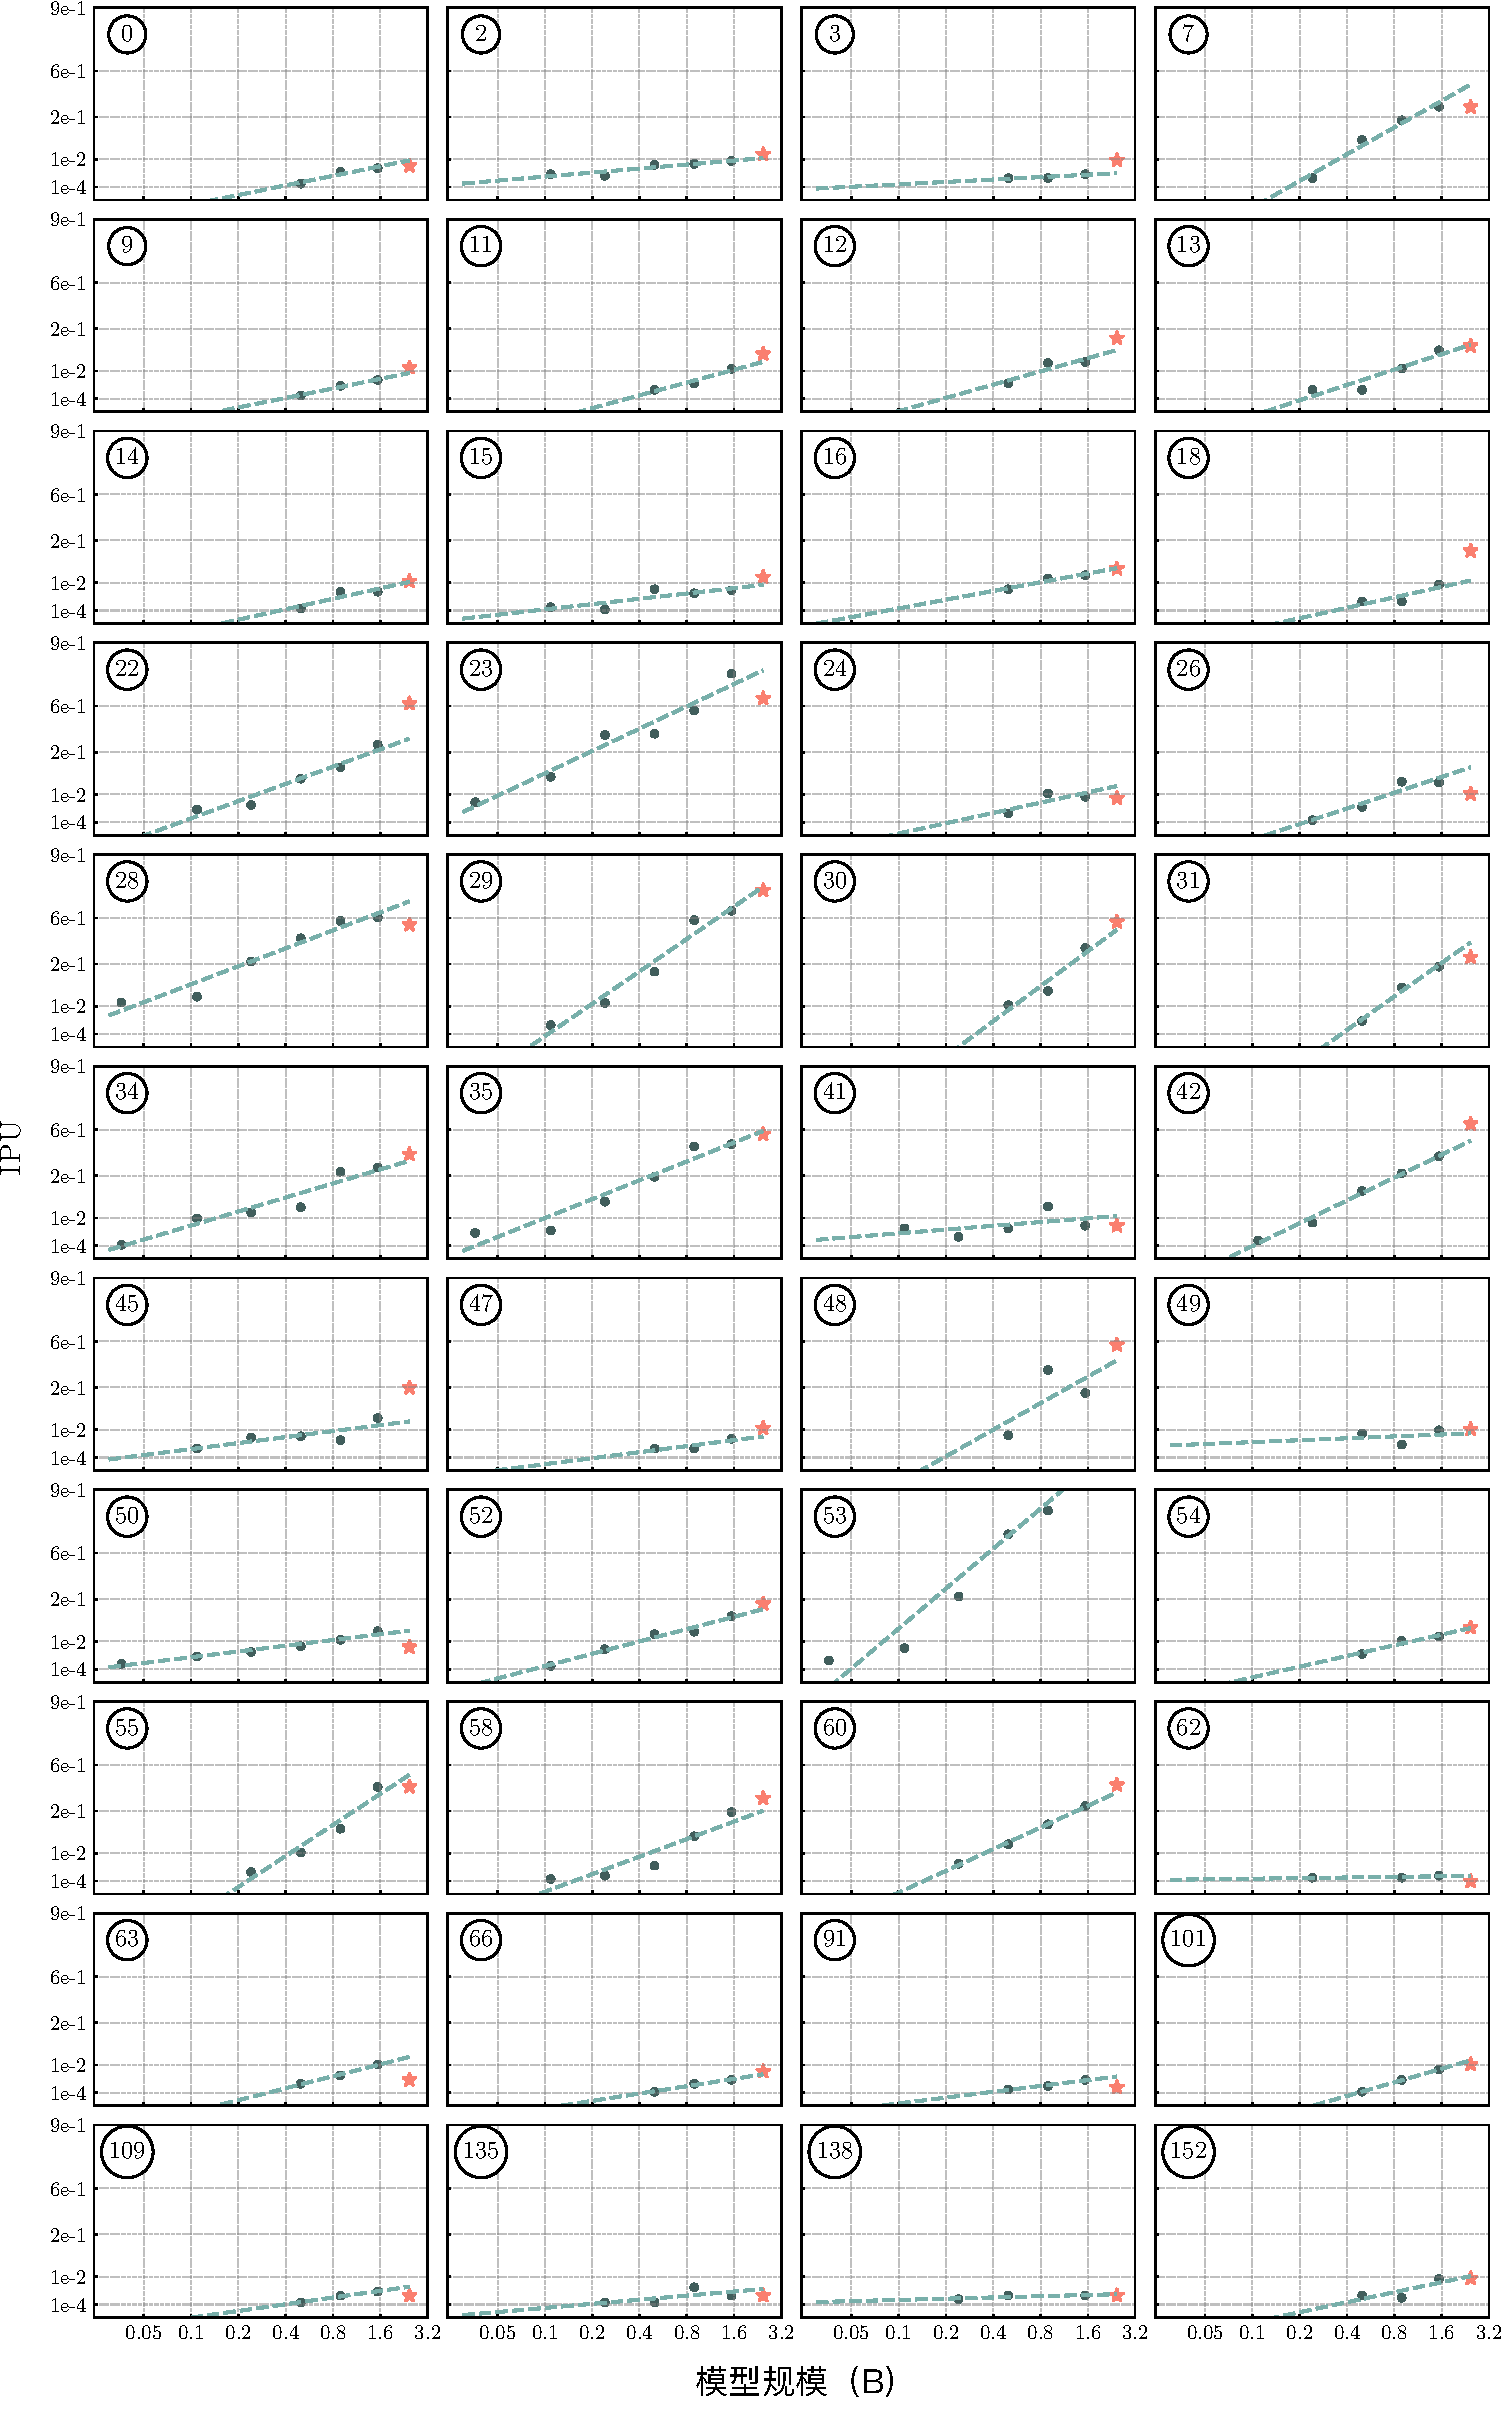
\includegraphics[width=0.85\textwidth]{pufigs/individual_passrate_vs_modelsize_part_main.zh.pdf}
  \caption{实例级扩展定律拟合结果}
  \label{fig:idp_with_modelsize_part1}
\end{figure}

\vspace{-0.3cm}
\section{S3Delta方法搜索结构的分数据集可视化。}


\label{app:heatmaps}
\begin{figure}[!htbp]
    \centering 
    \vspace{-0.3cm}
  \scalebox{0.74}{
% \hspace{-1em}
  \begin{subfigure}[t]{0.49\linewidth}
    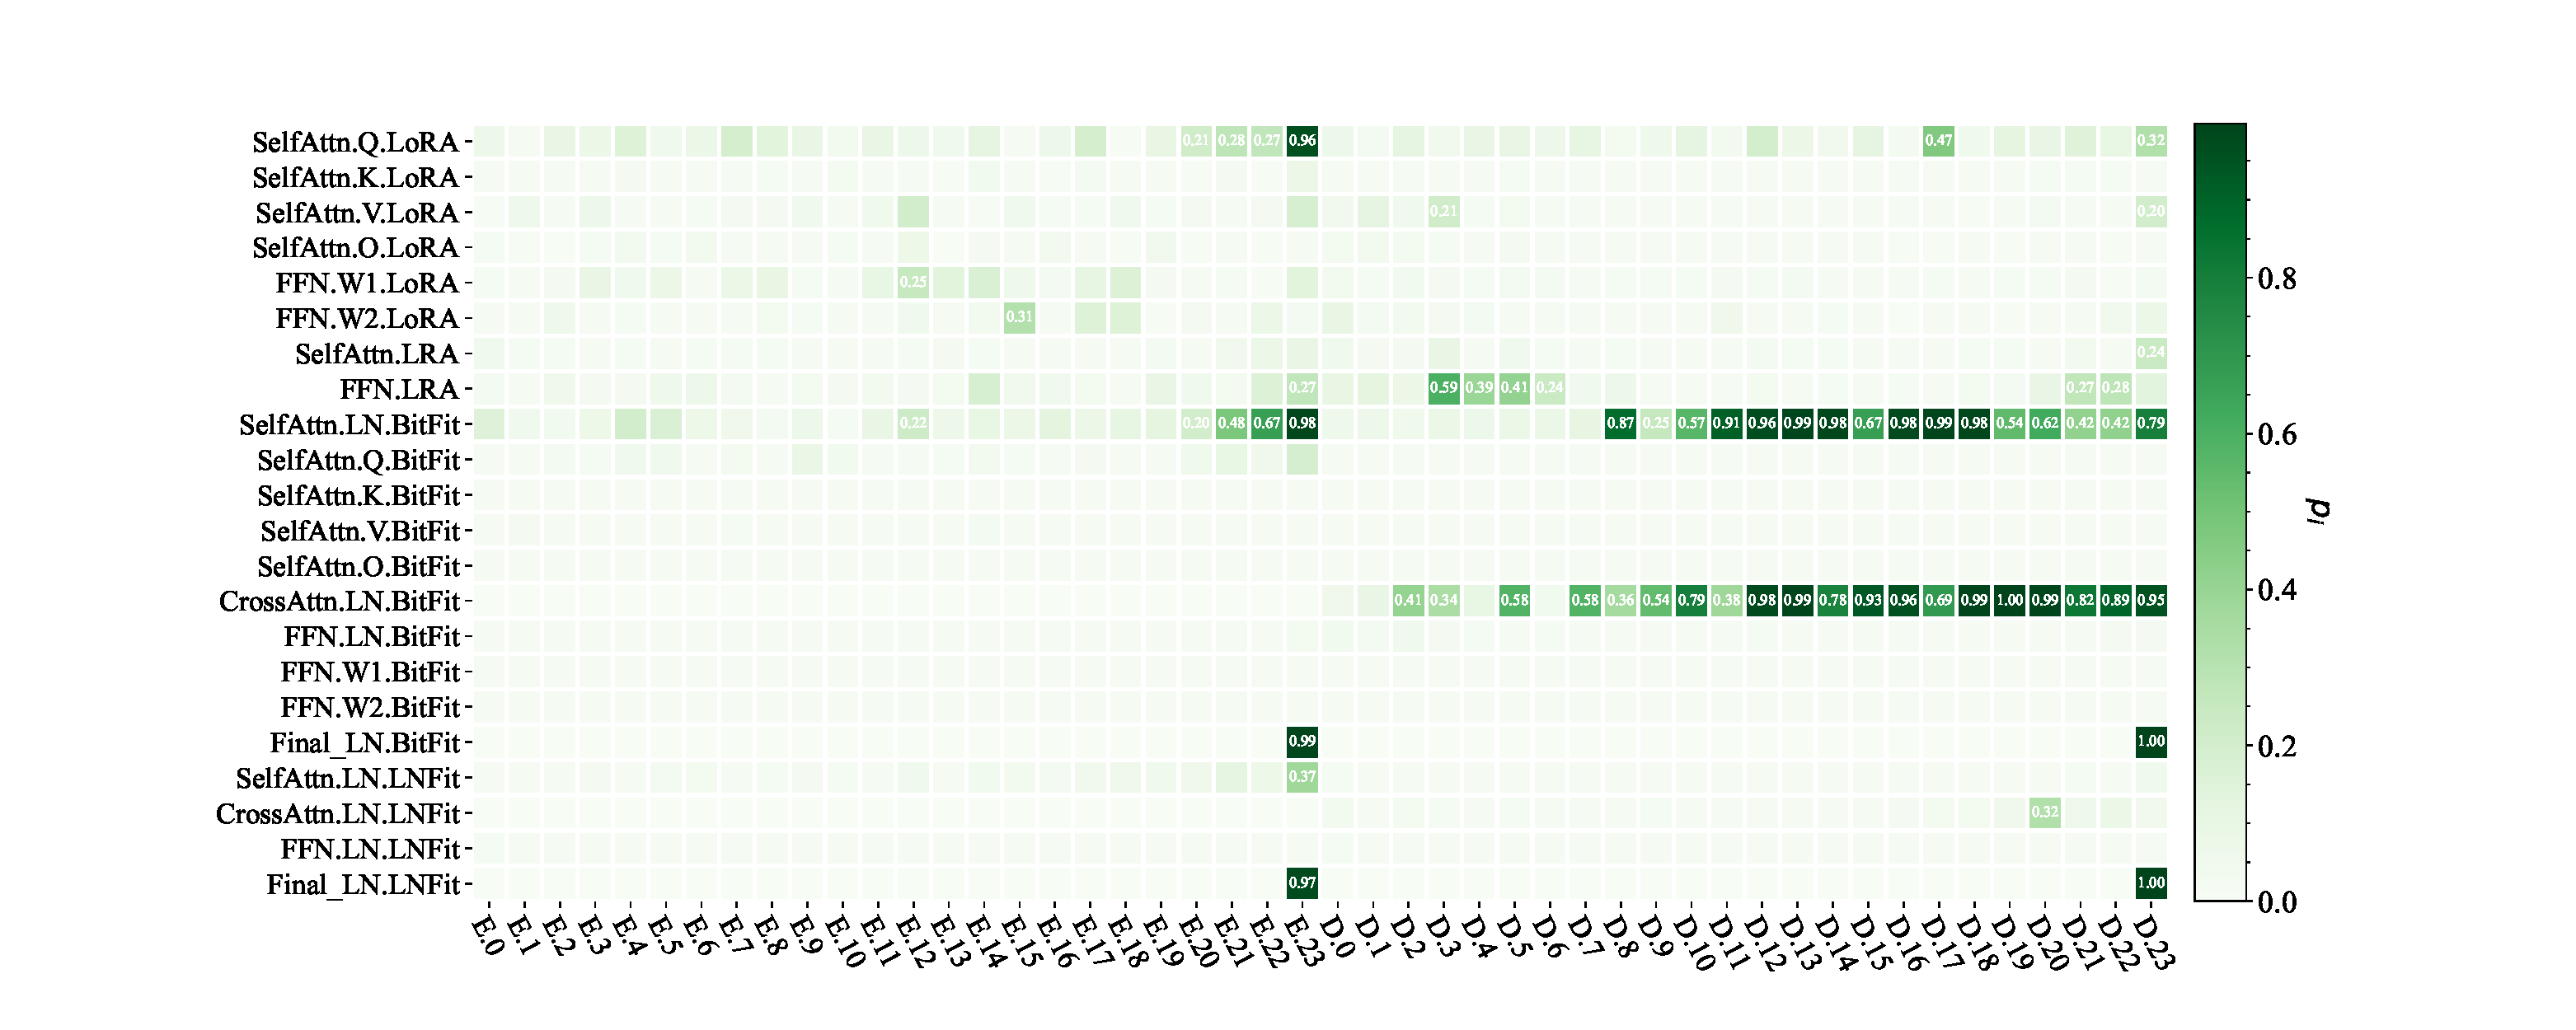
\includegraphics[width=\textwidth]{s3dfigs/heatmap_mix_1.389/cola_sparsity_1.389_heatmap.pdf} 
    \vspace{-0.45cm}
    \caption{CoLA}
  \end{subfigure}
  \begin{subfigure}[t]{0.49\textwidth}
    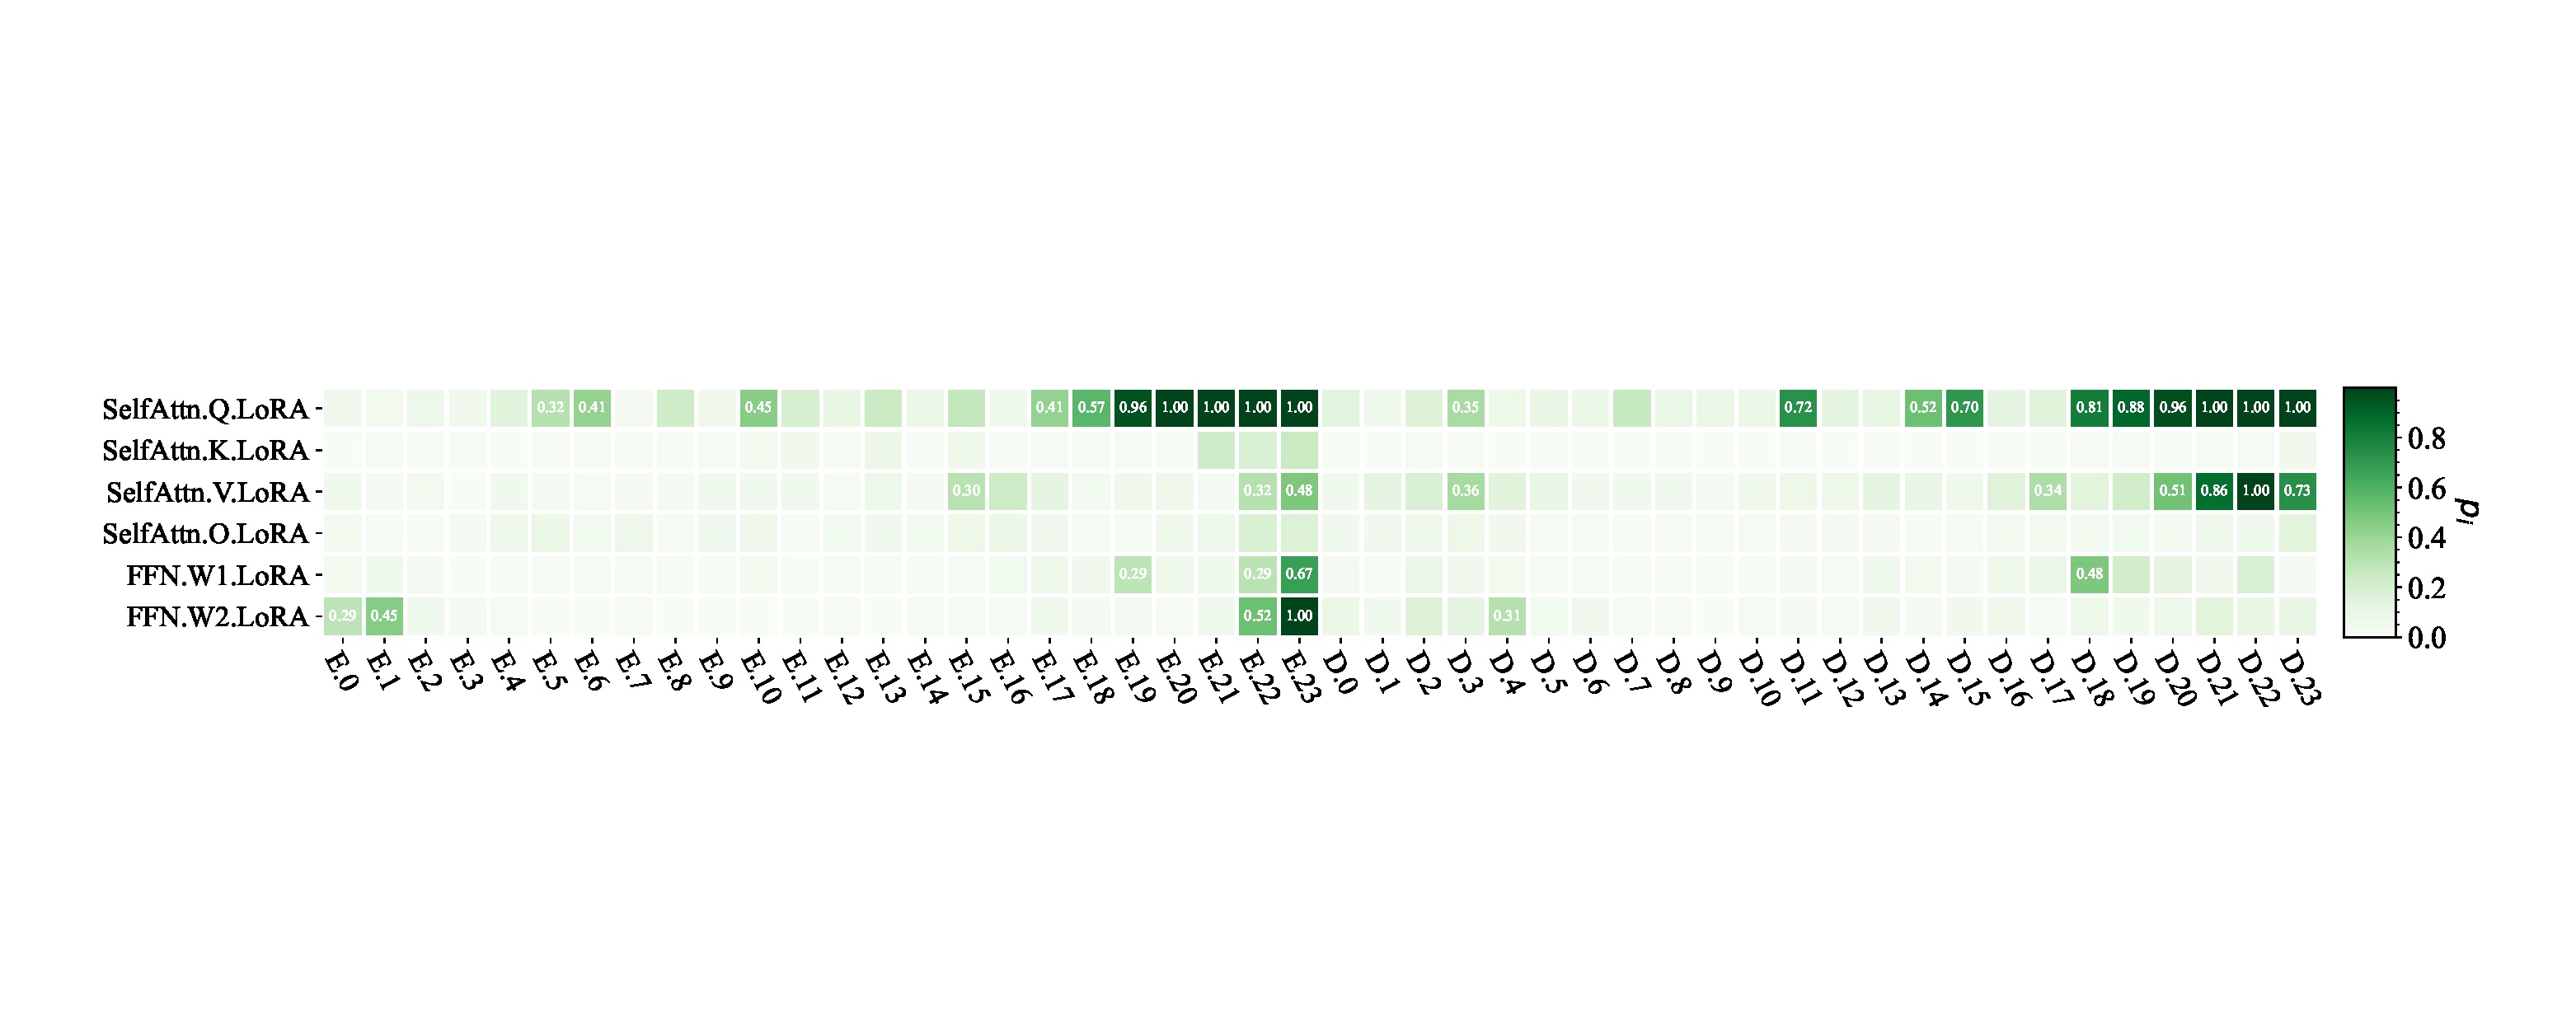
\includegraphics[width=\textwidth]{s3dfigs/heatmap_mix_1.389/mnli_sparsity_1.389_heatmap.pdf}
    \vspace{-0.45cm}
    \caption{MNLI}
  \end{subfigure}
  }
  \quad
  \scalebox{0.74}{
  \begin{subfigure}[t]{0.49\textwidth}
    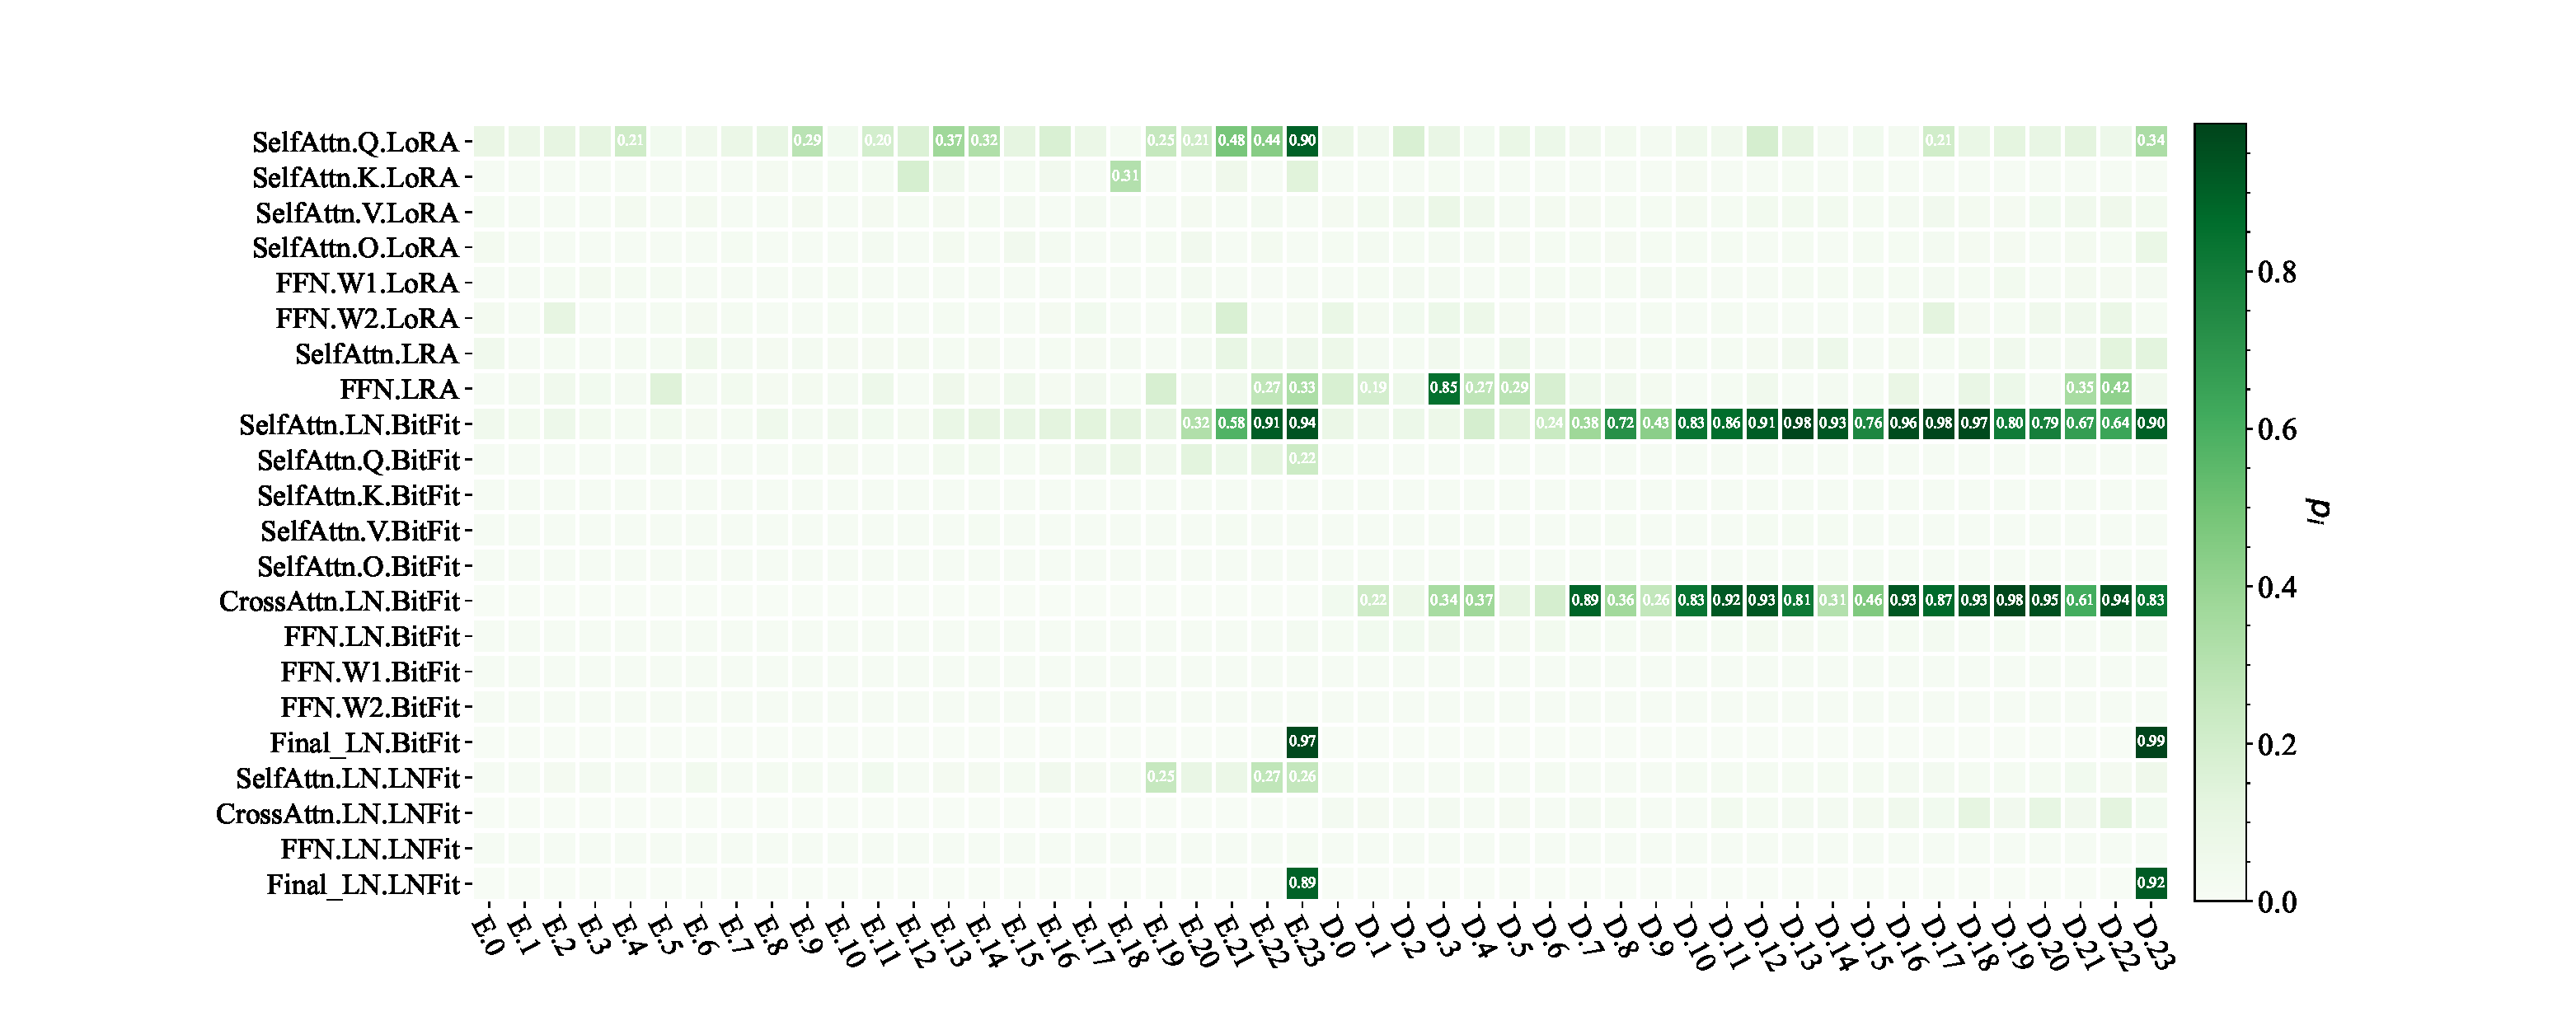
\includegraphics[width=\textwidth]{s3dfigs/heatmap_mix_1.389/mrpc_sparsity_1.389_heatmap.pdf}
    \vspace{-0.45cm}
    \caption{MRPC}
  \end{subfigure}
  \begin{subfigure}[t]{0.49\textwidth}
    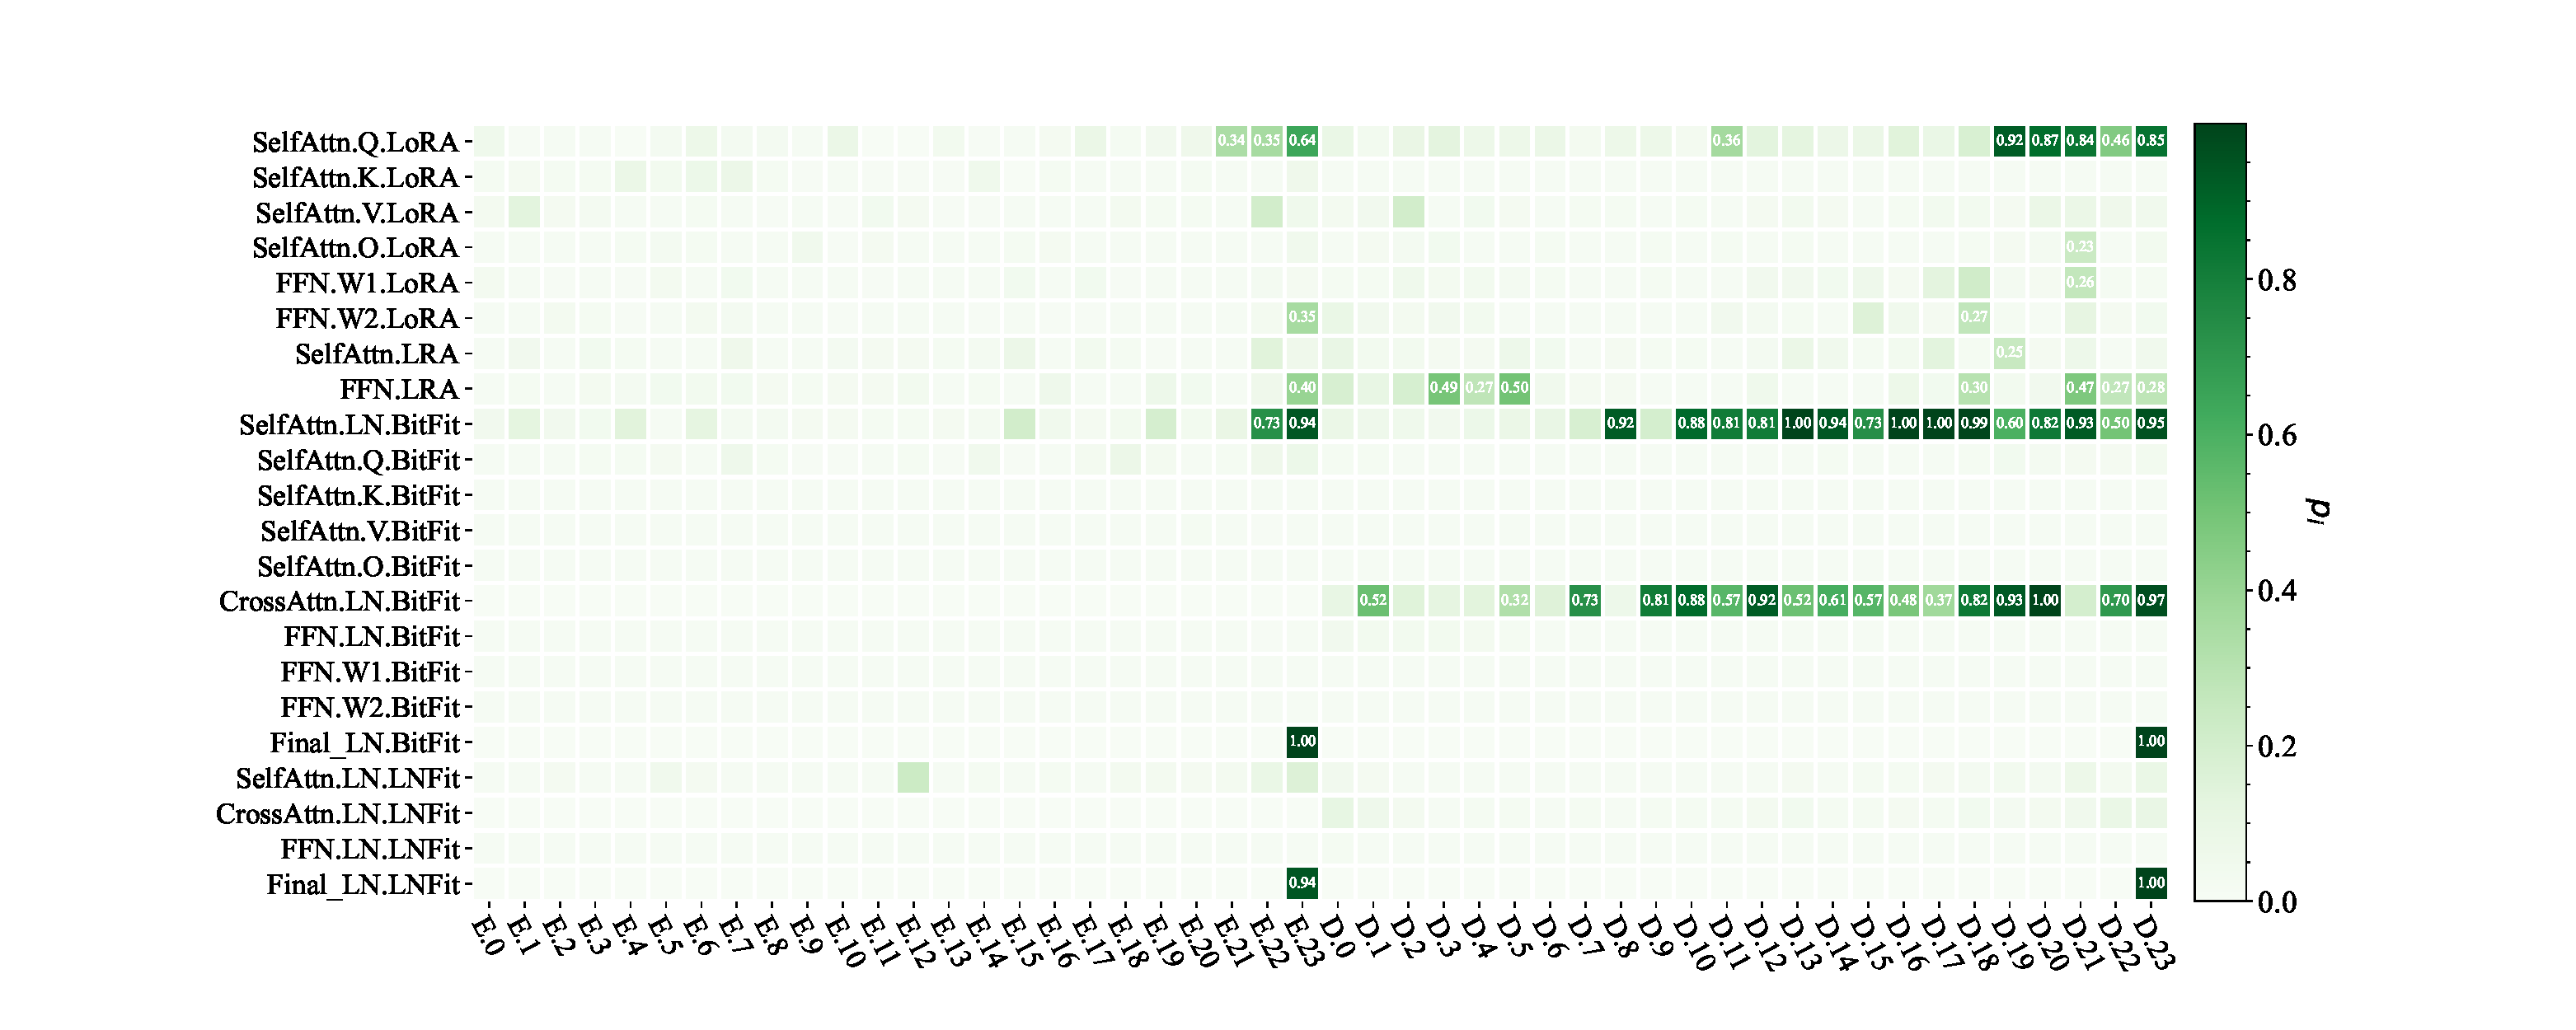
\includegraphics[width=\textwidth]{s3dfigs/heatmap_mix_1.389/qnli_sparsity_1.389_heatmap.pdf}
    \vspace{-0.45cm}
    \caption{QNLI}
  \end{subfigure}}
  \quad
  
  \scalebox{0.74}{
  \begin{subfigure}[t]{0.49\textwidth}
    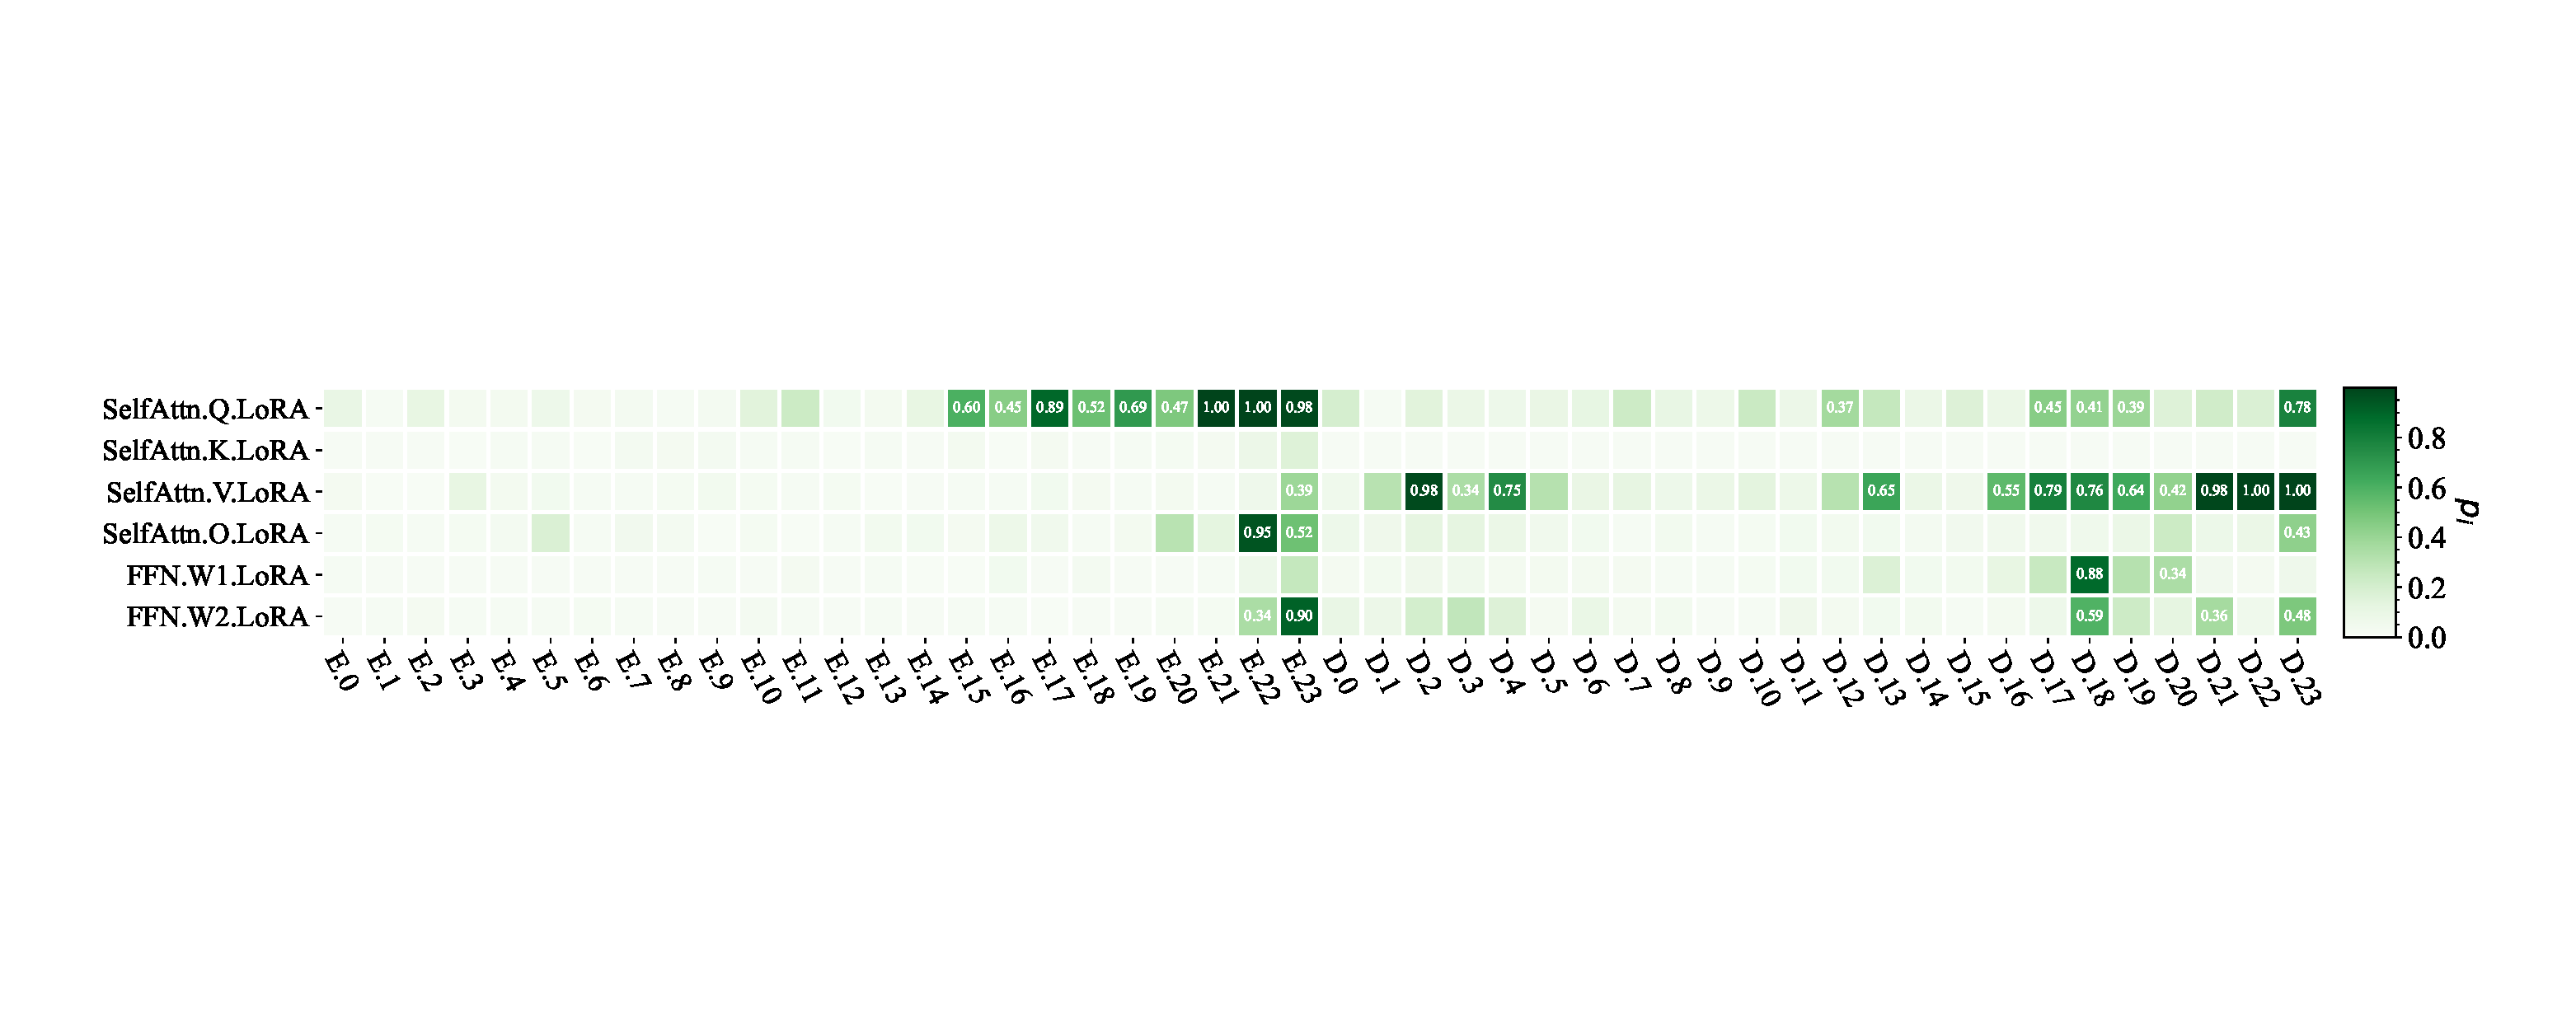
\includegraphics[width=\textwidth]{s3dfigs/heatmap_mix_1.389/qqp_sparsity_1.389_heatmap.pdf}
    \vspace{-0.45cm}
    \caption{QQP}
  \end{subfigure}
  \begin{subfigure}[t]{0.49\textwidth}

    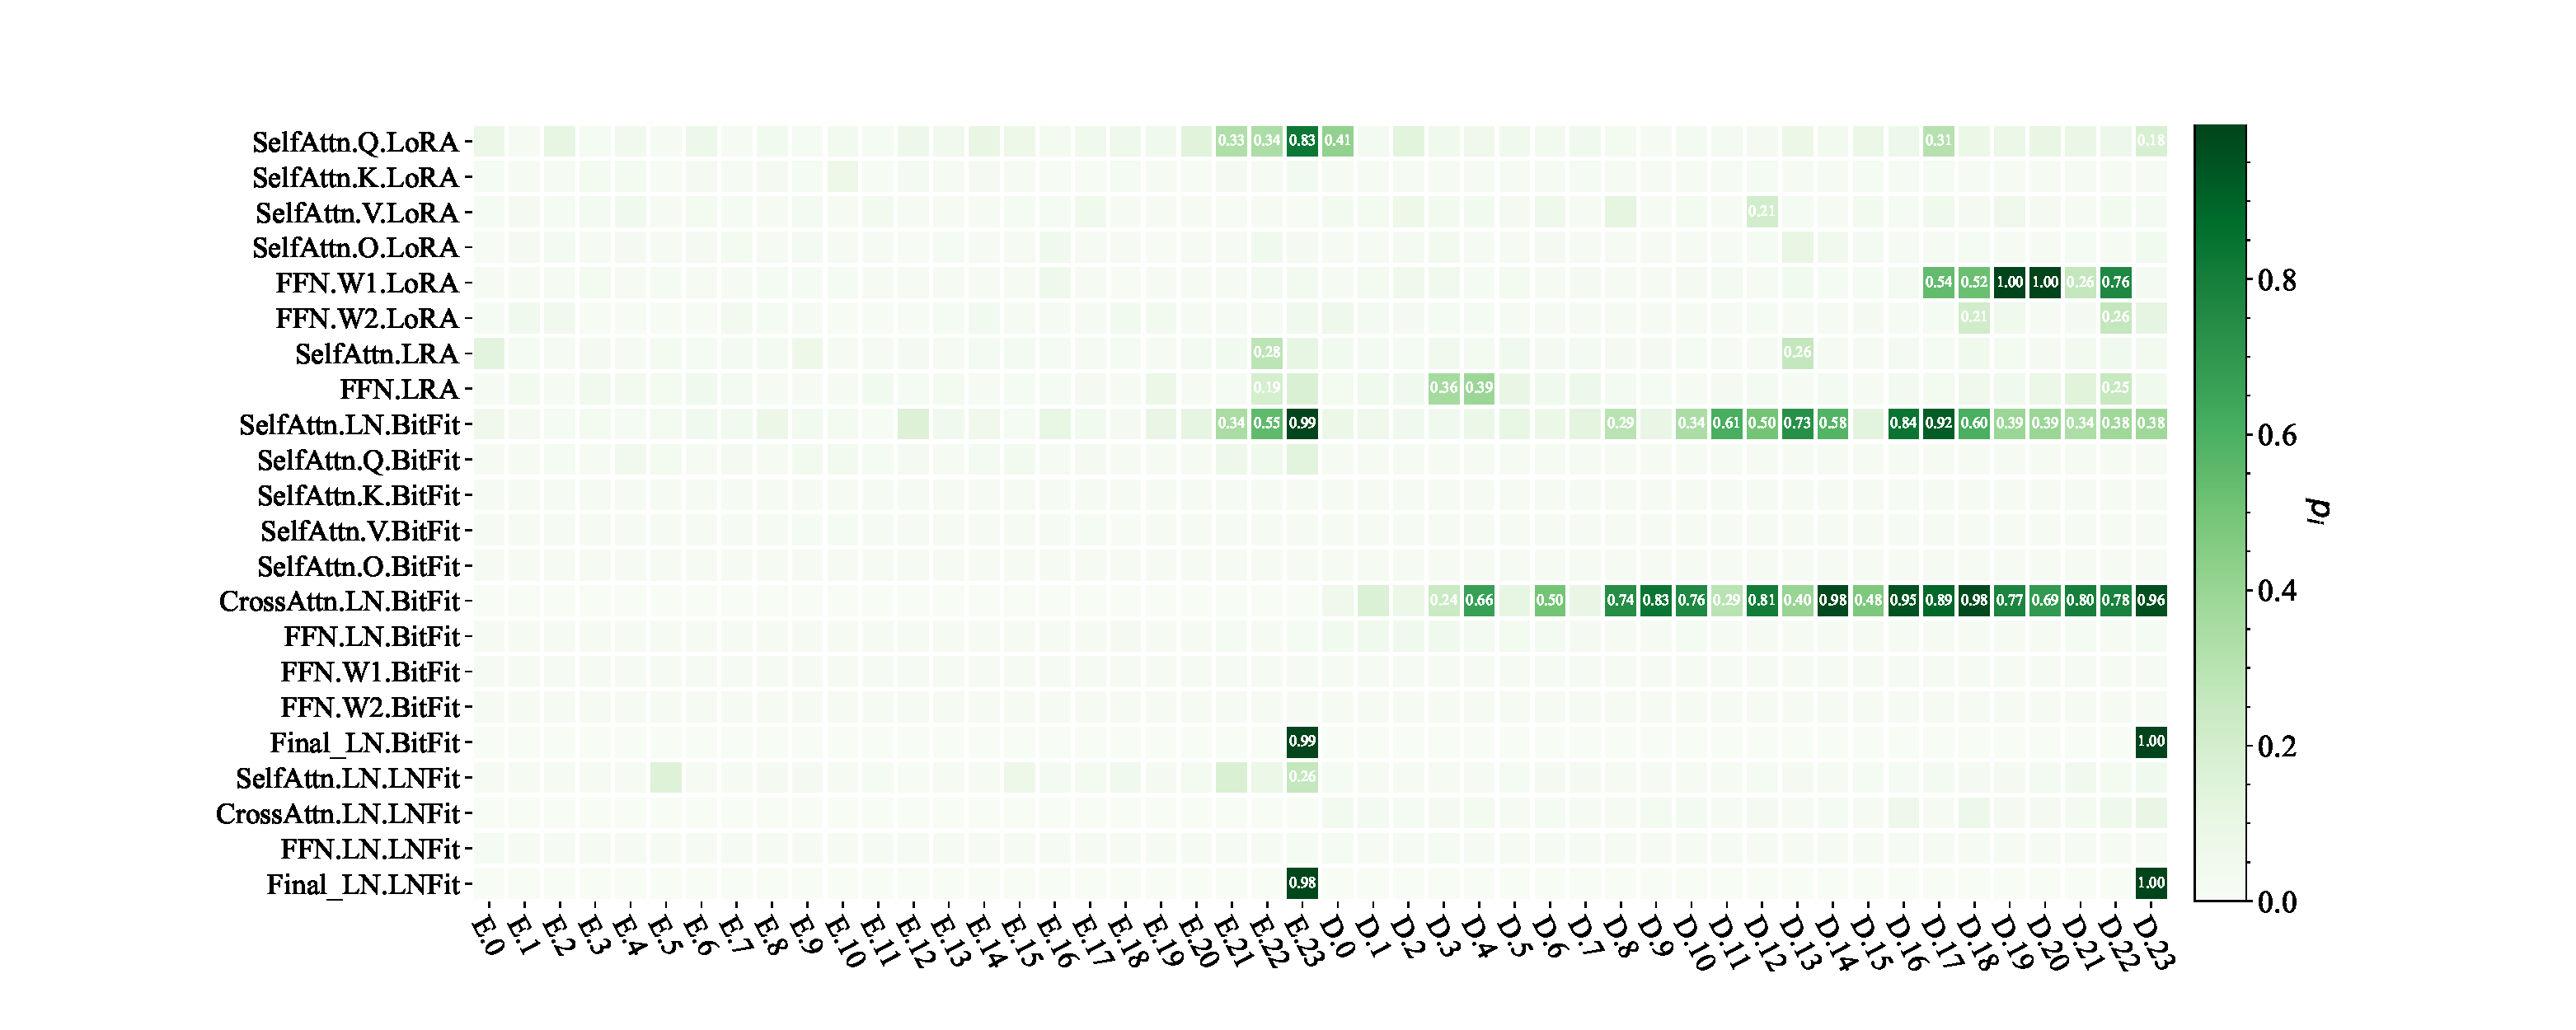
\includegraphics[width=\textwidth]{s3dfigs/heatmap_mix_1.389/sst2_sparsity_1.389_heatmap.pdf}
    \vspace{-0.45cm}
    \caption{SST2}
  \end{subfigure}}
  \quad

  \scalebox{0.74}{
  \begin{subfigure}[t]{0.49\textwidth}
    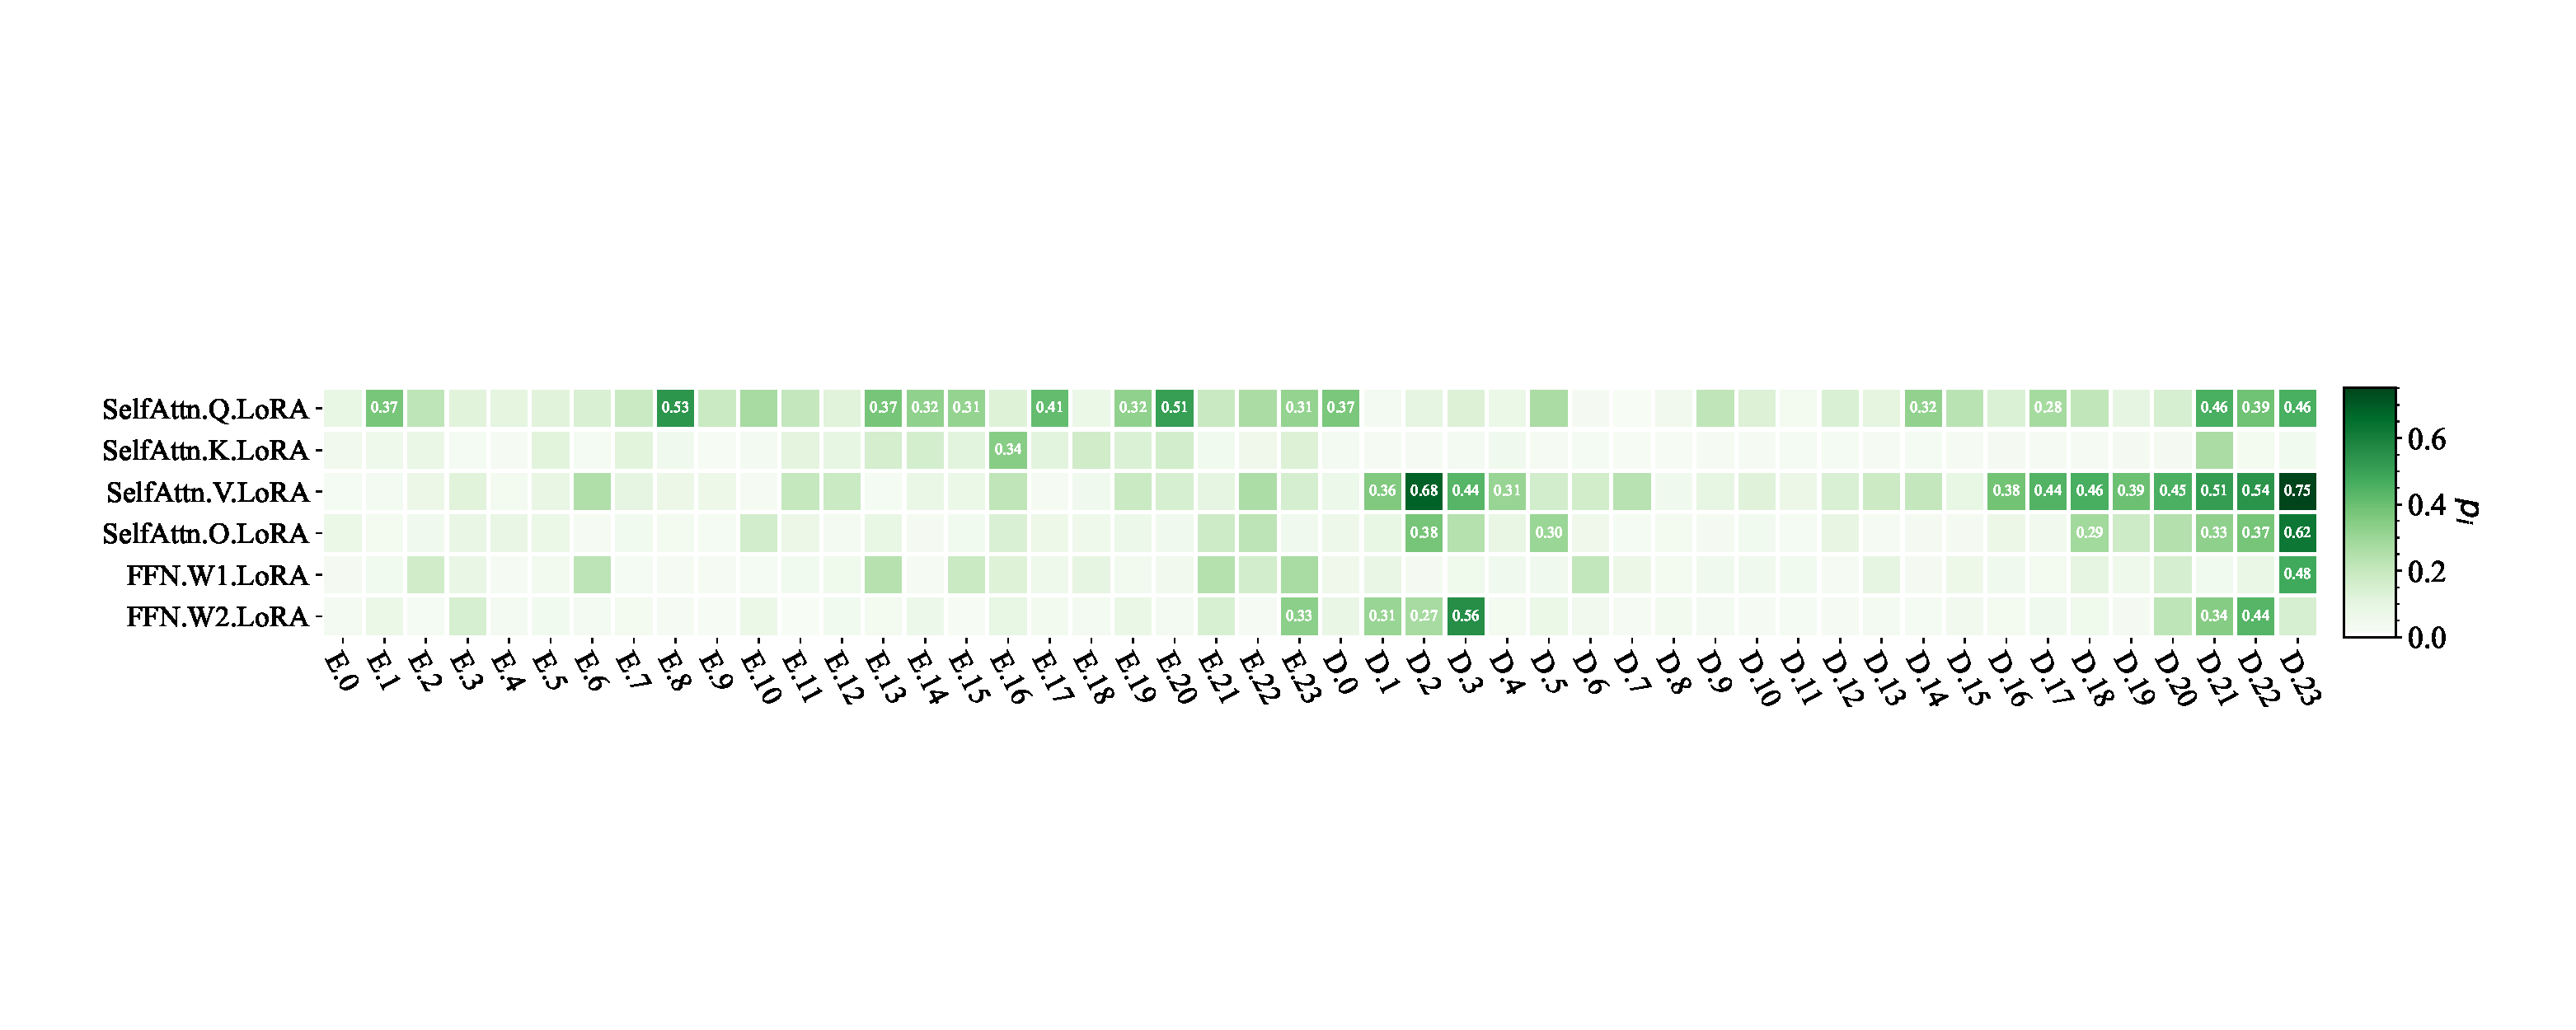
\includegraphics[width=\textwidth]{s3dfigs/heatmap_mix_1.389/stsb_sparsity_1.389_heatmap.pdf}
    \vspace{-0.45cm}
    \caption{STSB}
  \end{subfigure}
  \begin{subfigure}[t]{0.49\textwidth}
    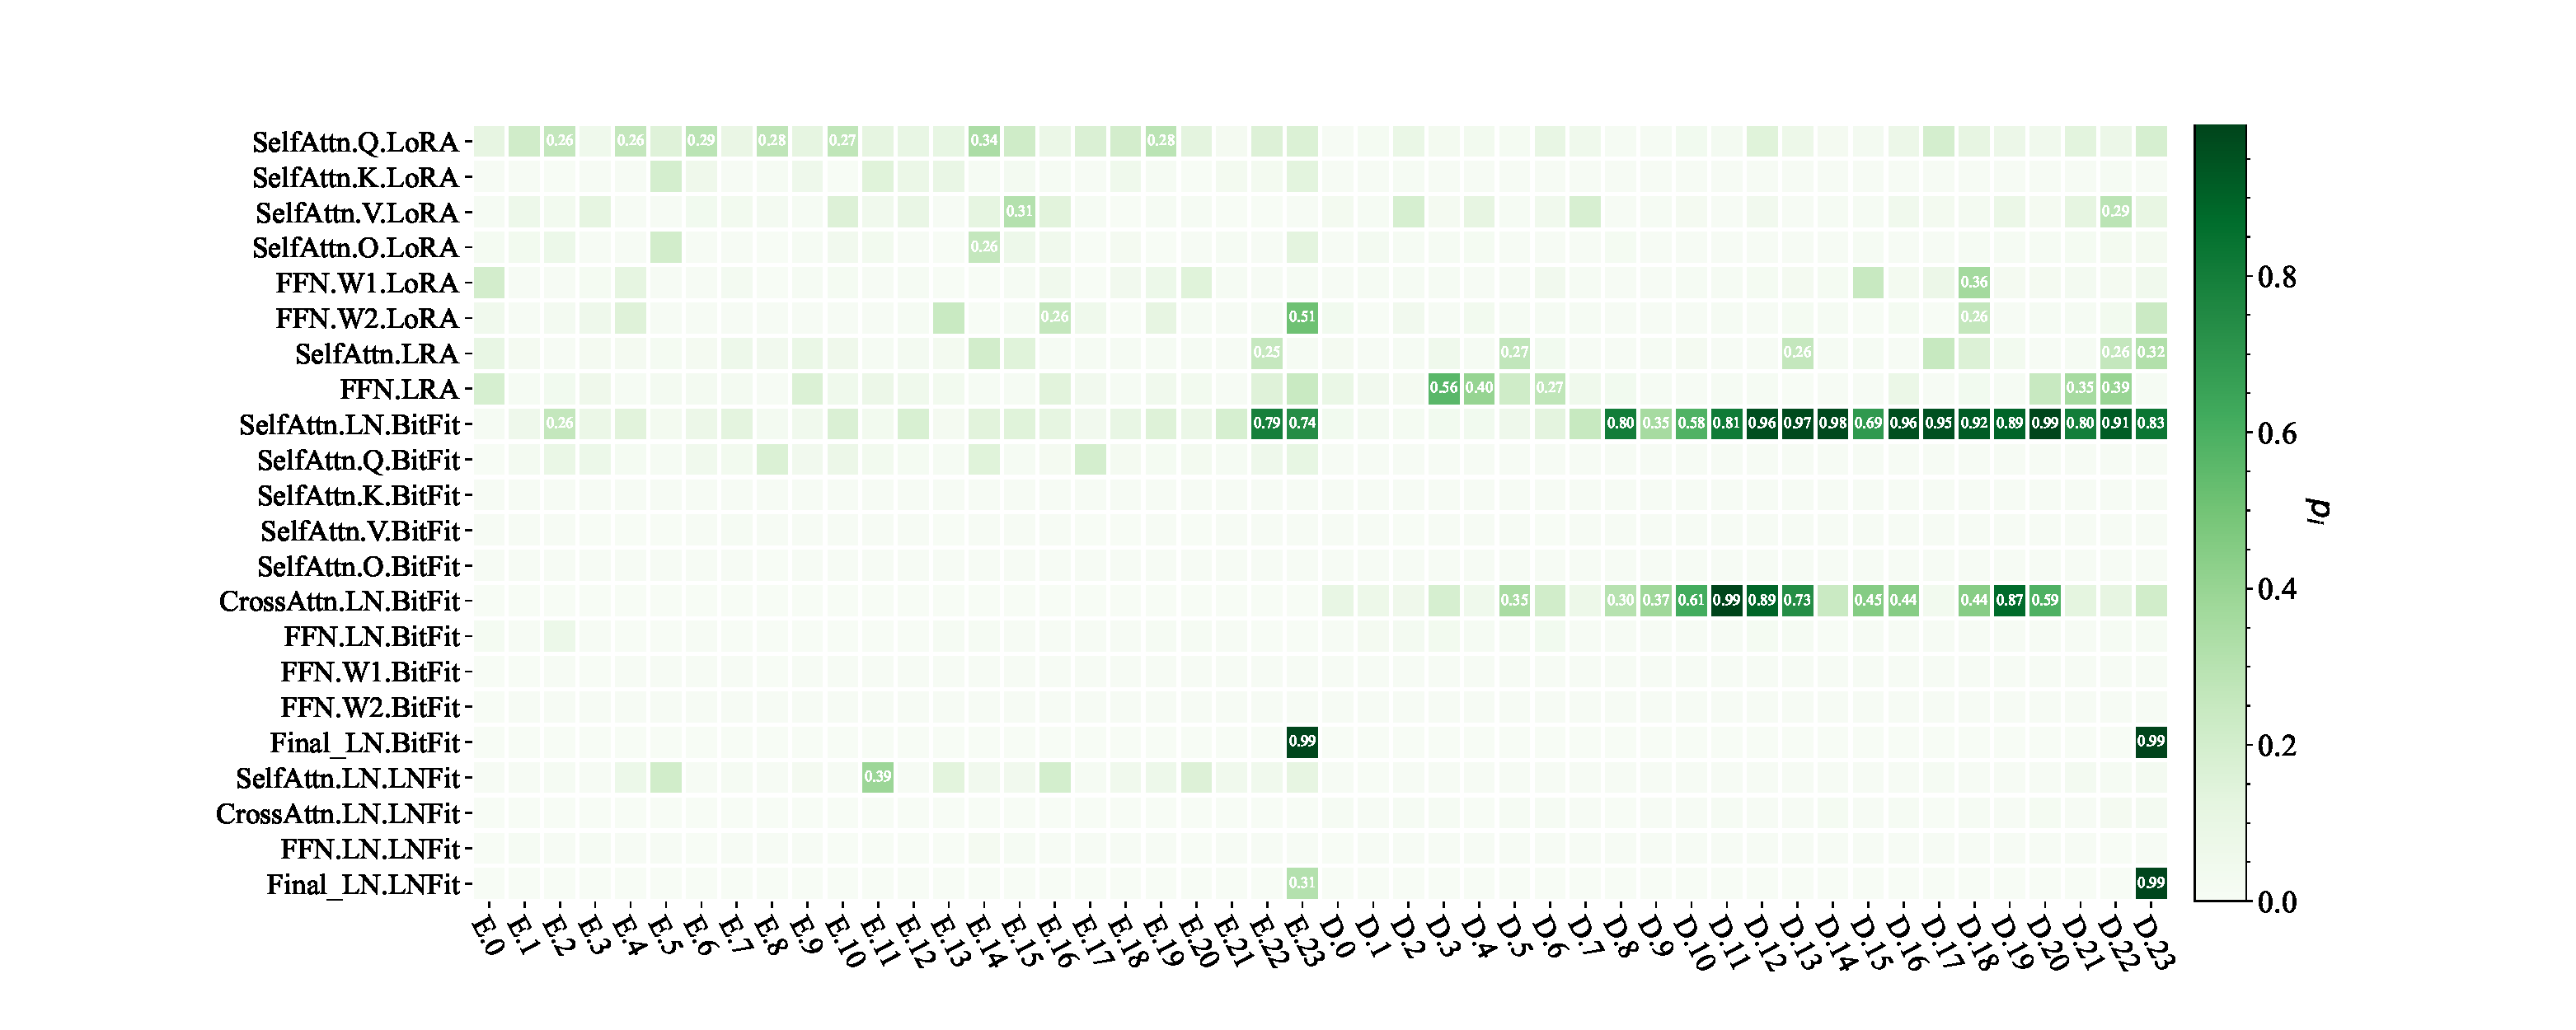
\includegraphics[width=\textwidth]{s3dfigs/heatmap_mix_1.389/superglue-boolq_sparsity_1.389_heatmap.pdf}
    \vspace{-0.45cm}
    \caption{BoolQ}
  \end{subfigure}}
  \quad
  
  \scalebox{0.74}{
  \begin{subfigure}[t]{0.49\textwidth}
    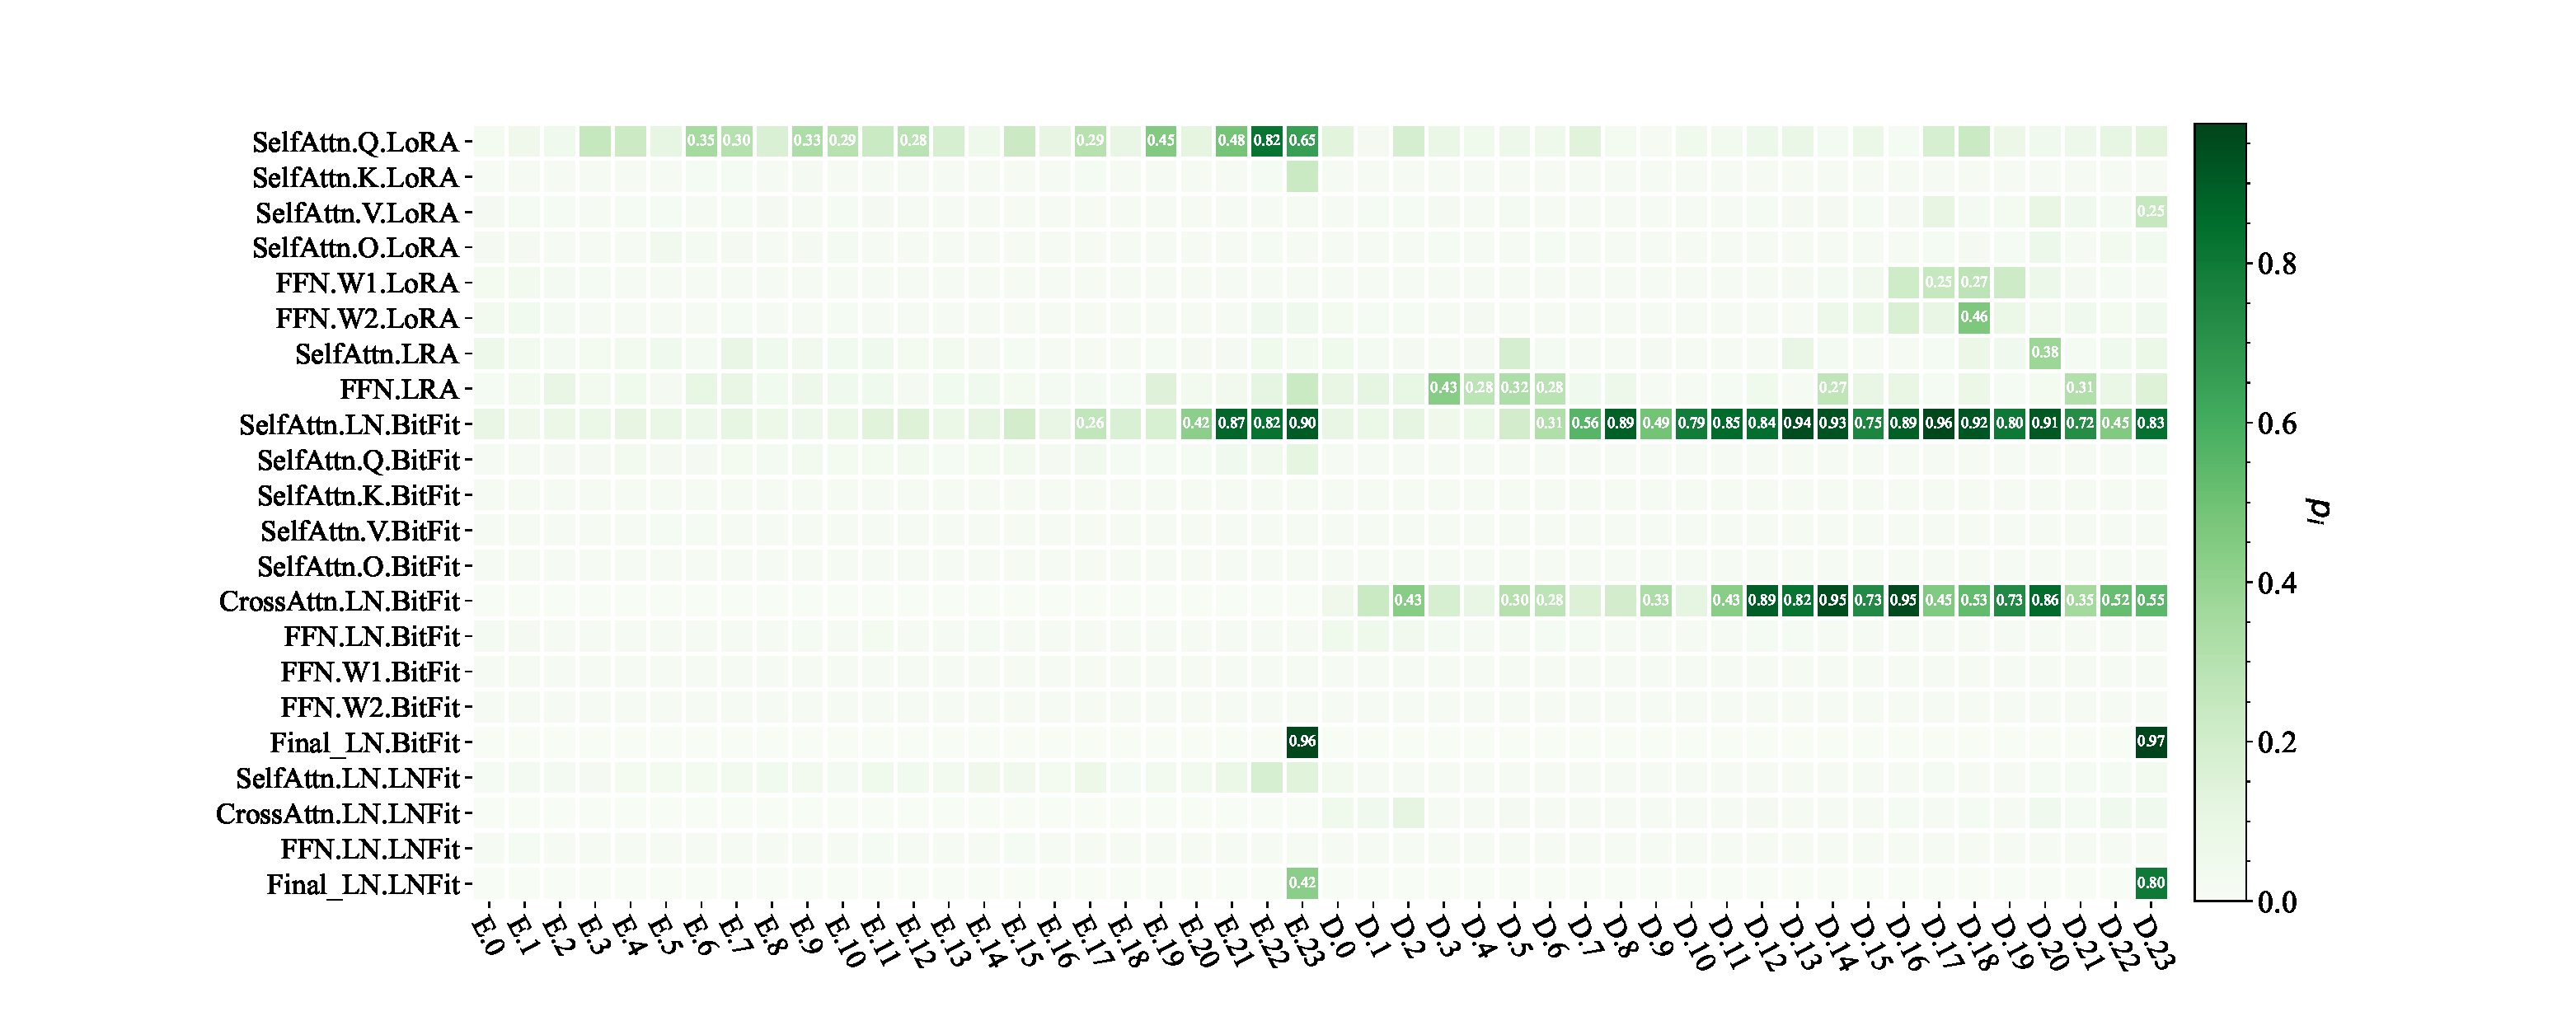
\includegraphics[width=\textwidth]{s3dfigs/heatmap_mix_1.389/superglue-cb_sparsity_1.389_heatmap.pdf}
    \vspace{-0.45cm}
    \caption{CB}
  \end{subfigure}
  \begin{subfigure}[t]{0.49\textwidth}
    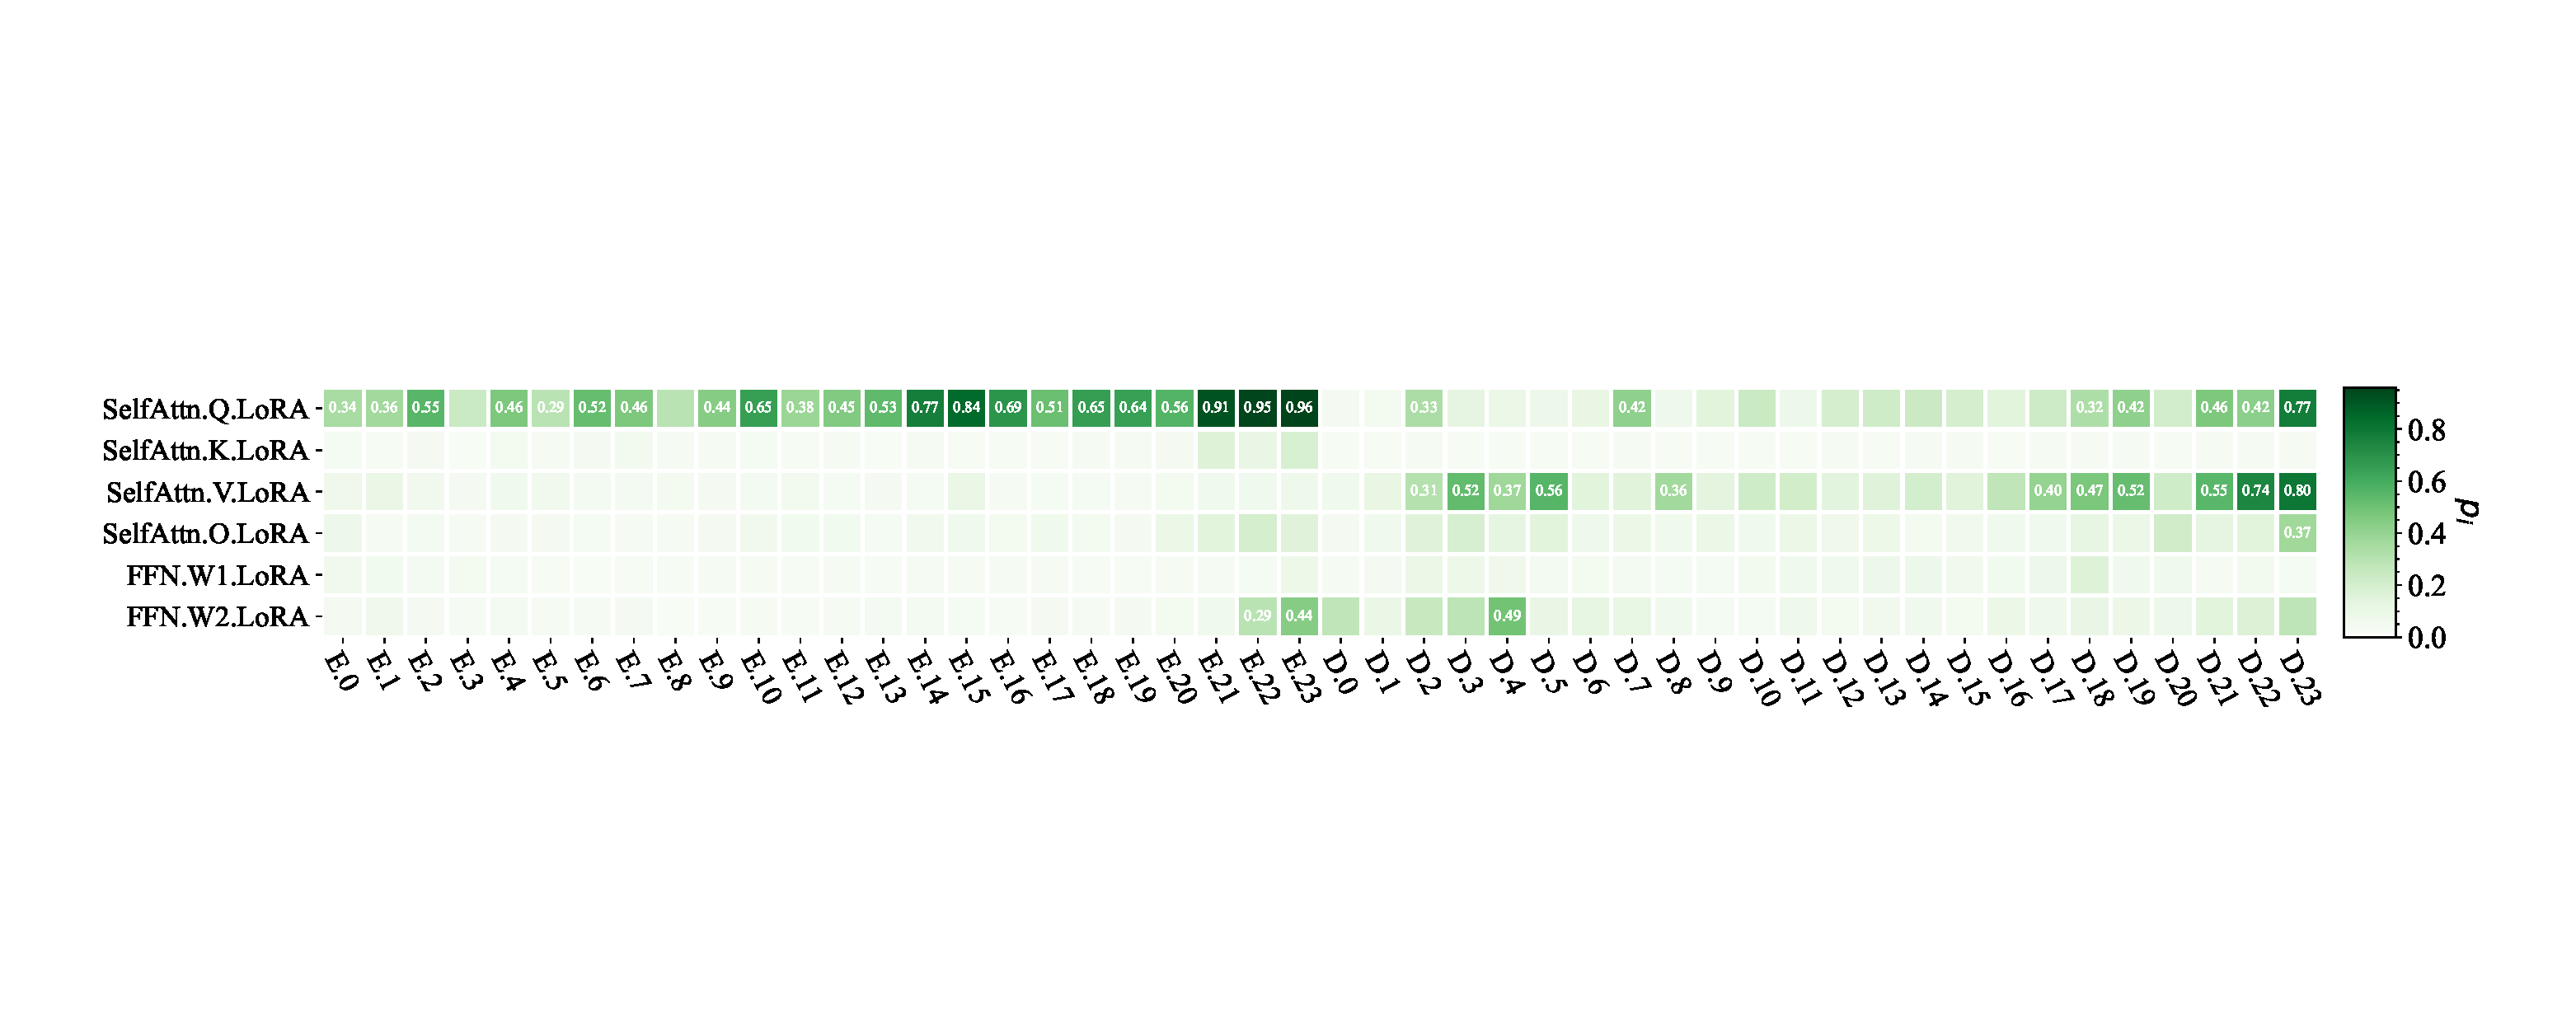
\includegraphics[width=\textwidth]{s3dfigs/heatmap_mix_1.389/superglue-copa_sparsity_1.389_heatmap.pdf}
    \vspace{-0.45cm}
    \caption{COPA}
  \end{subfigure}}
  \quad
  
  \scalebox{0.74}{
  \begin{subfigure}[t]{0.49\textwidth}
    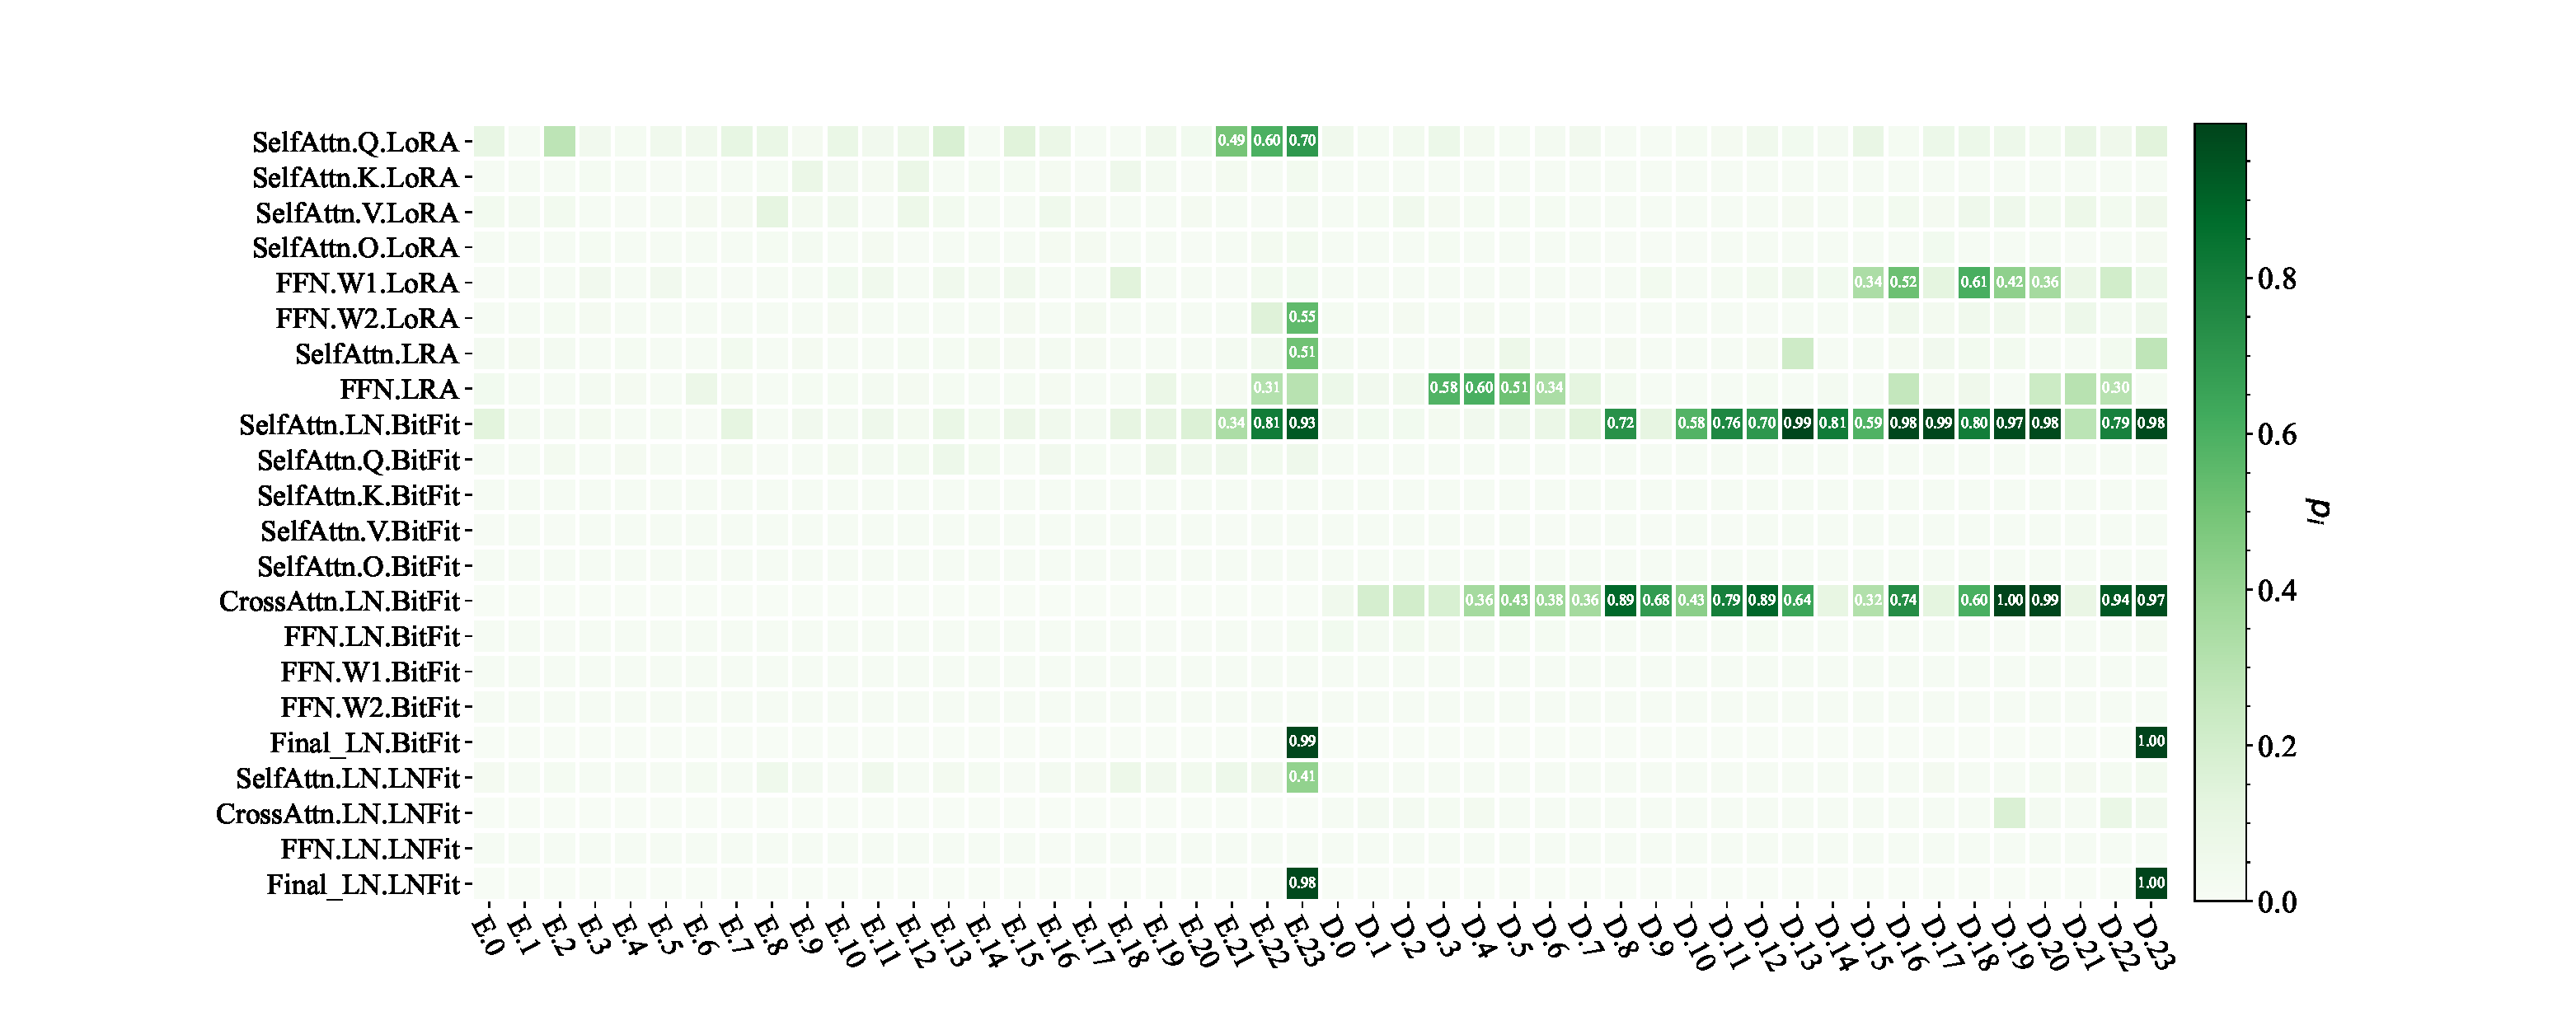
\includegraphics[width=\textwidth]{s3dfigs/heatmap_mix_1.389/superglue-multirc_sparsity_1.389_heatmap.pdf}
    \vspace{-0.45cm}
    \caption{MultiRC}
  \end{subfigure}
  \begin{subfigure}[t]{0.49\textwidth}
    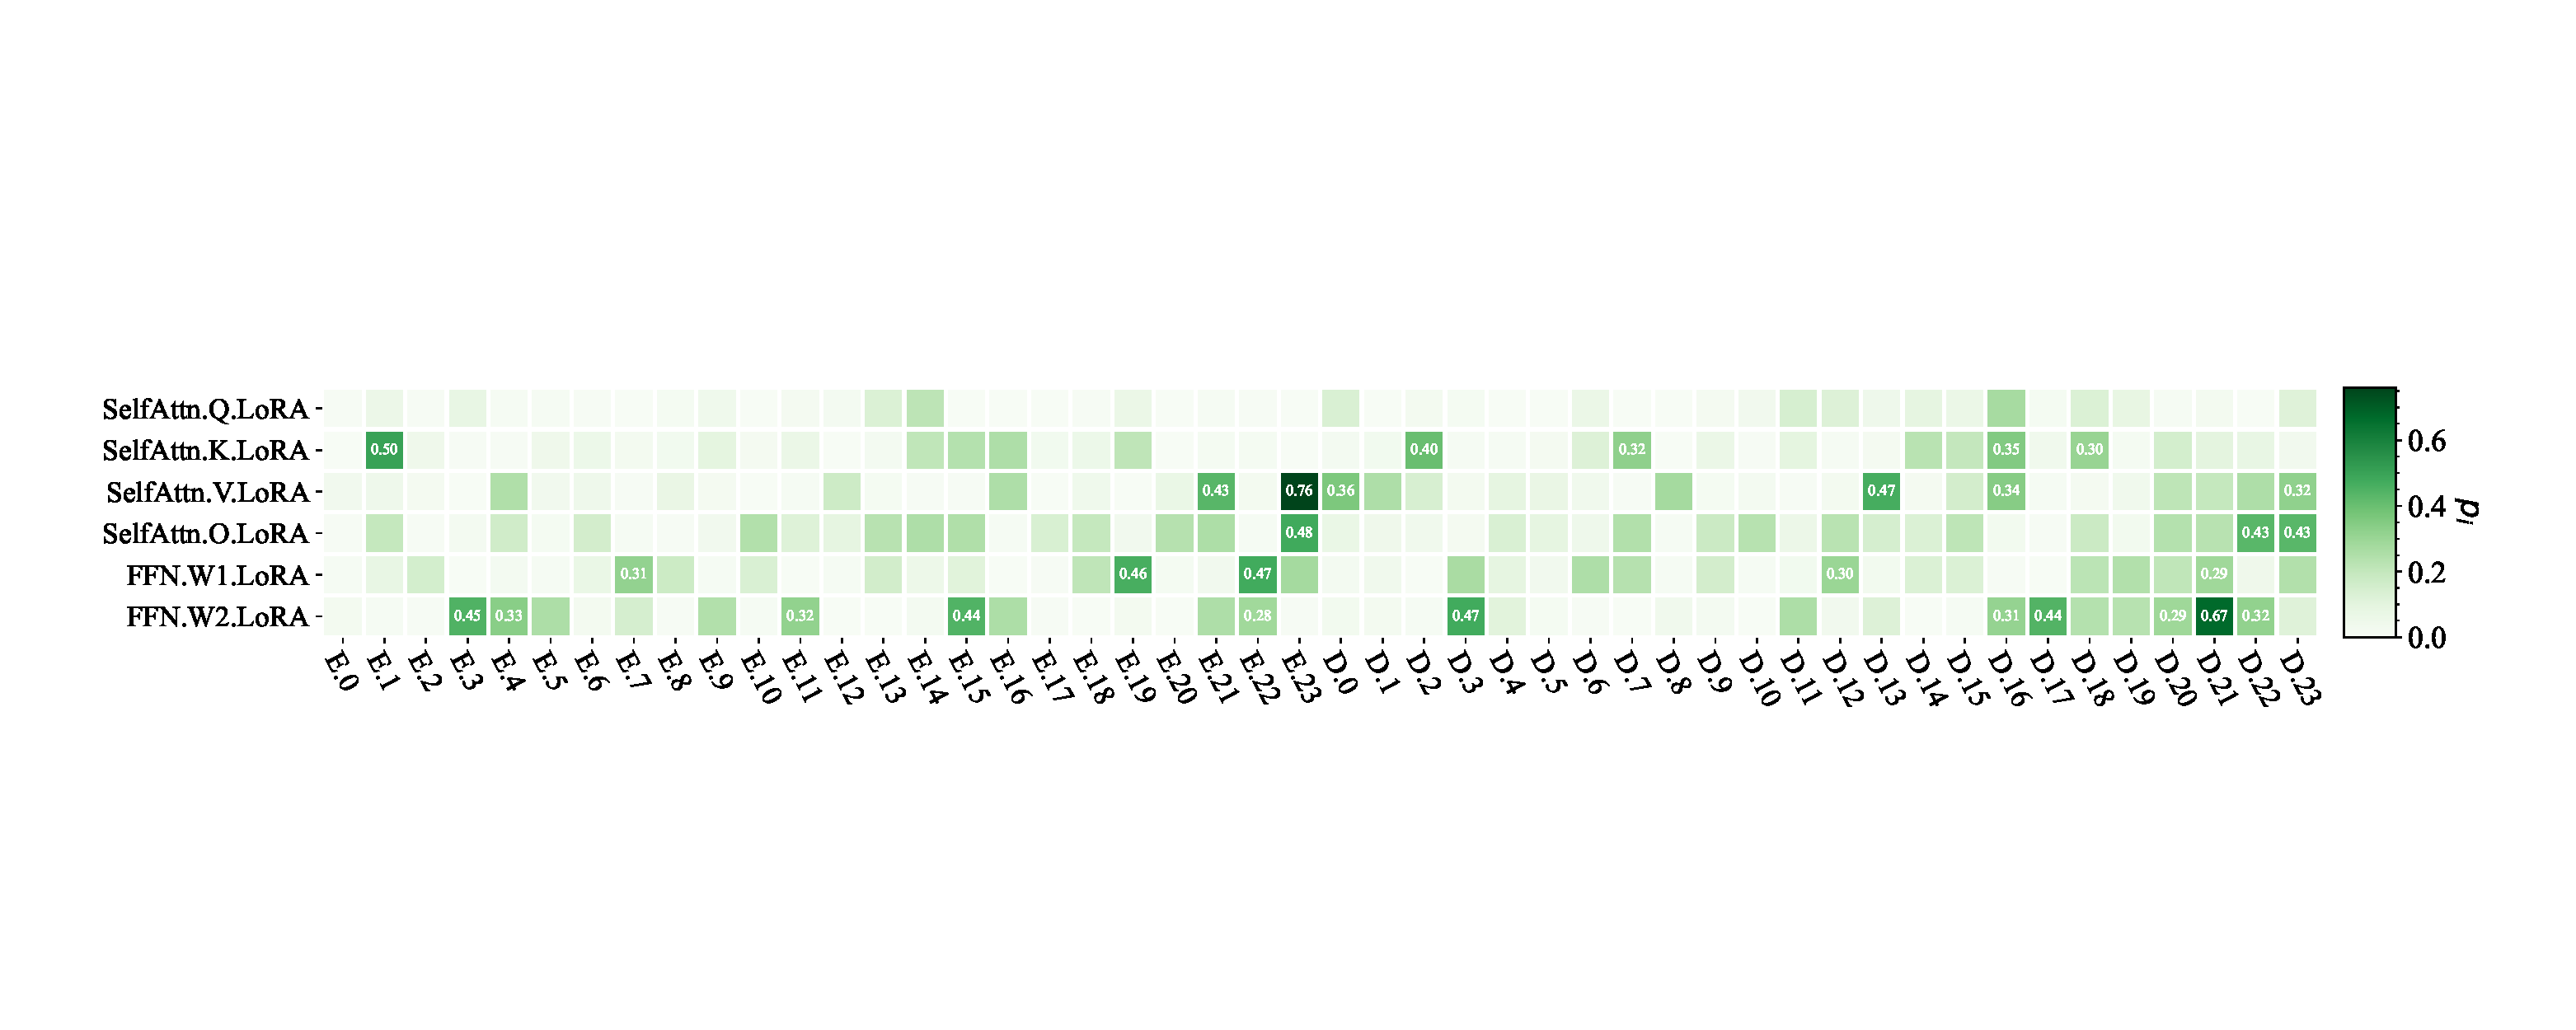
\includegraphics[width=\textwidth]{s3dfigs/heatmap_mix_1.389/superglue-record_sparsity_1.389_heatmap.pdf}
    \vspace{-0.45cm}
    \caption{ReCoRD}
  \end{subfigure}}
  \quad
  
  \scalebox{0.74}{
  \begin{subfigure}[t]{0.49\textwidth}
    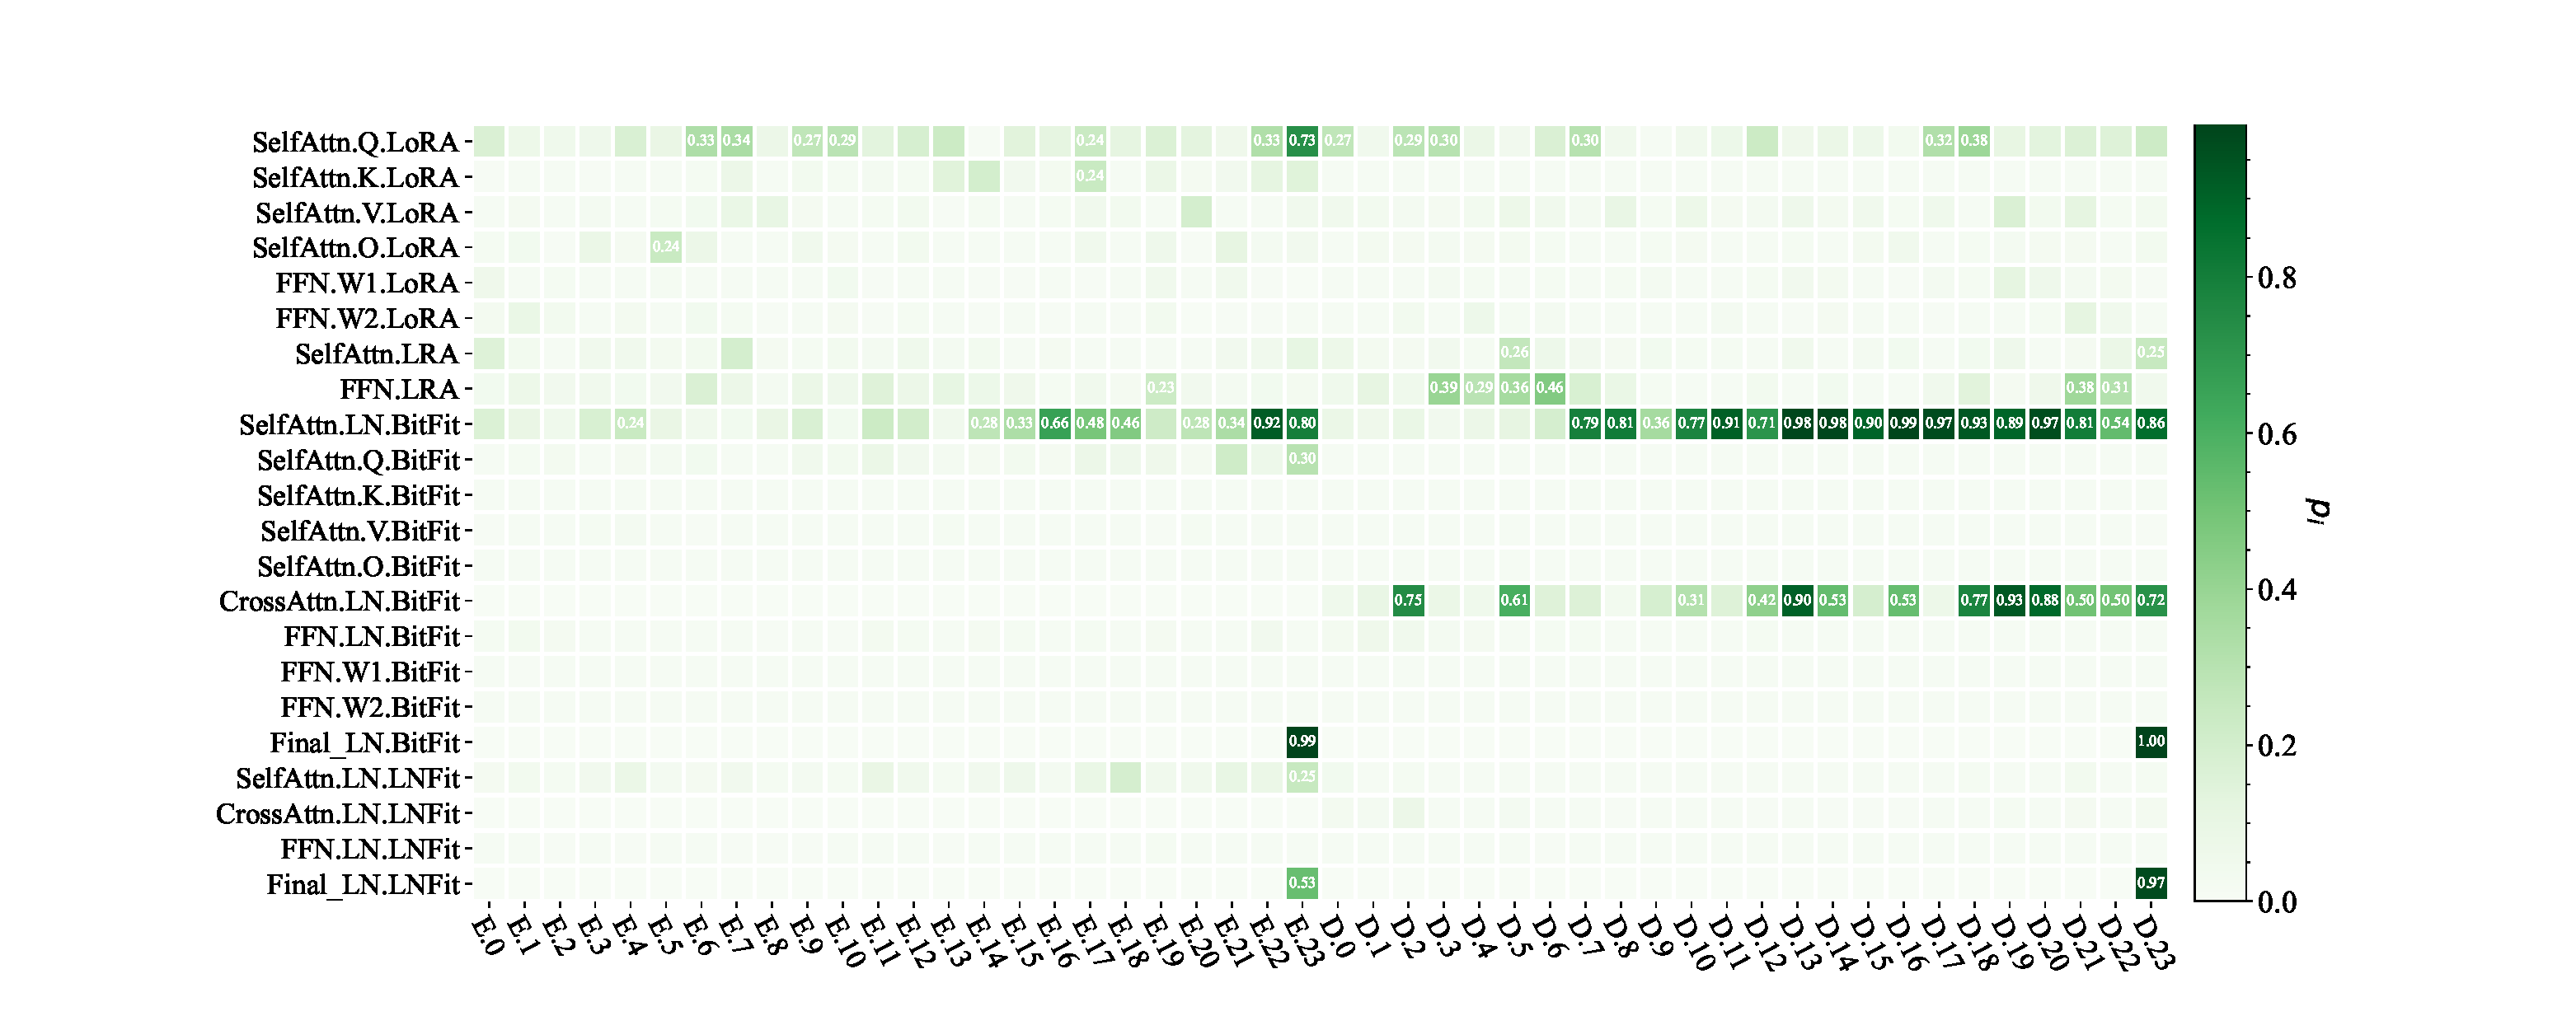
\includegraphics[width=\textwidth]{s3dfigs/heatmap_mix_1.389/superglue-rte_sparsity_1.389_heatmap.pdf}
    \vspace{-0.45cm}
    \caption{RTE}
  \end{subfigure}
  \begin{subfigure}[t]{0.49\textwidth}
    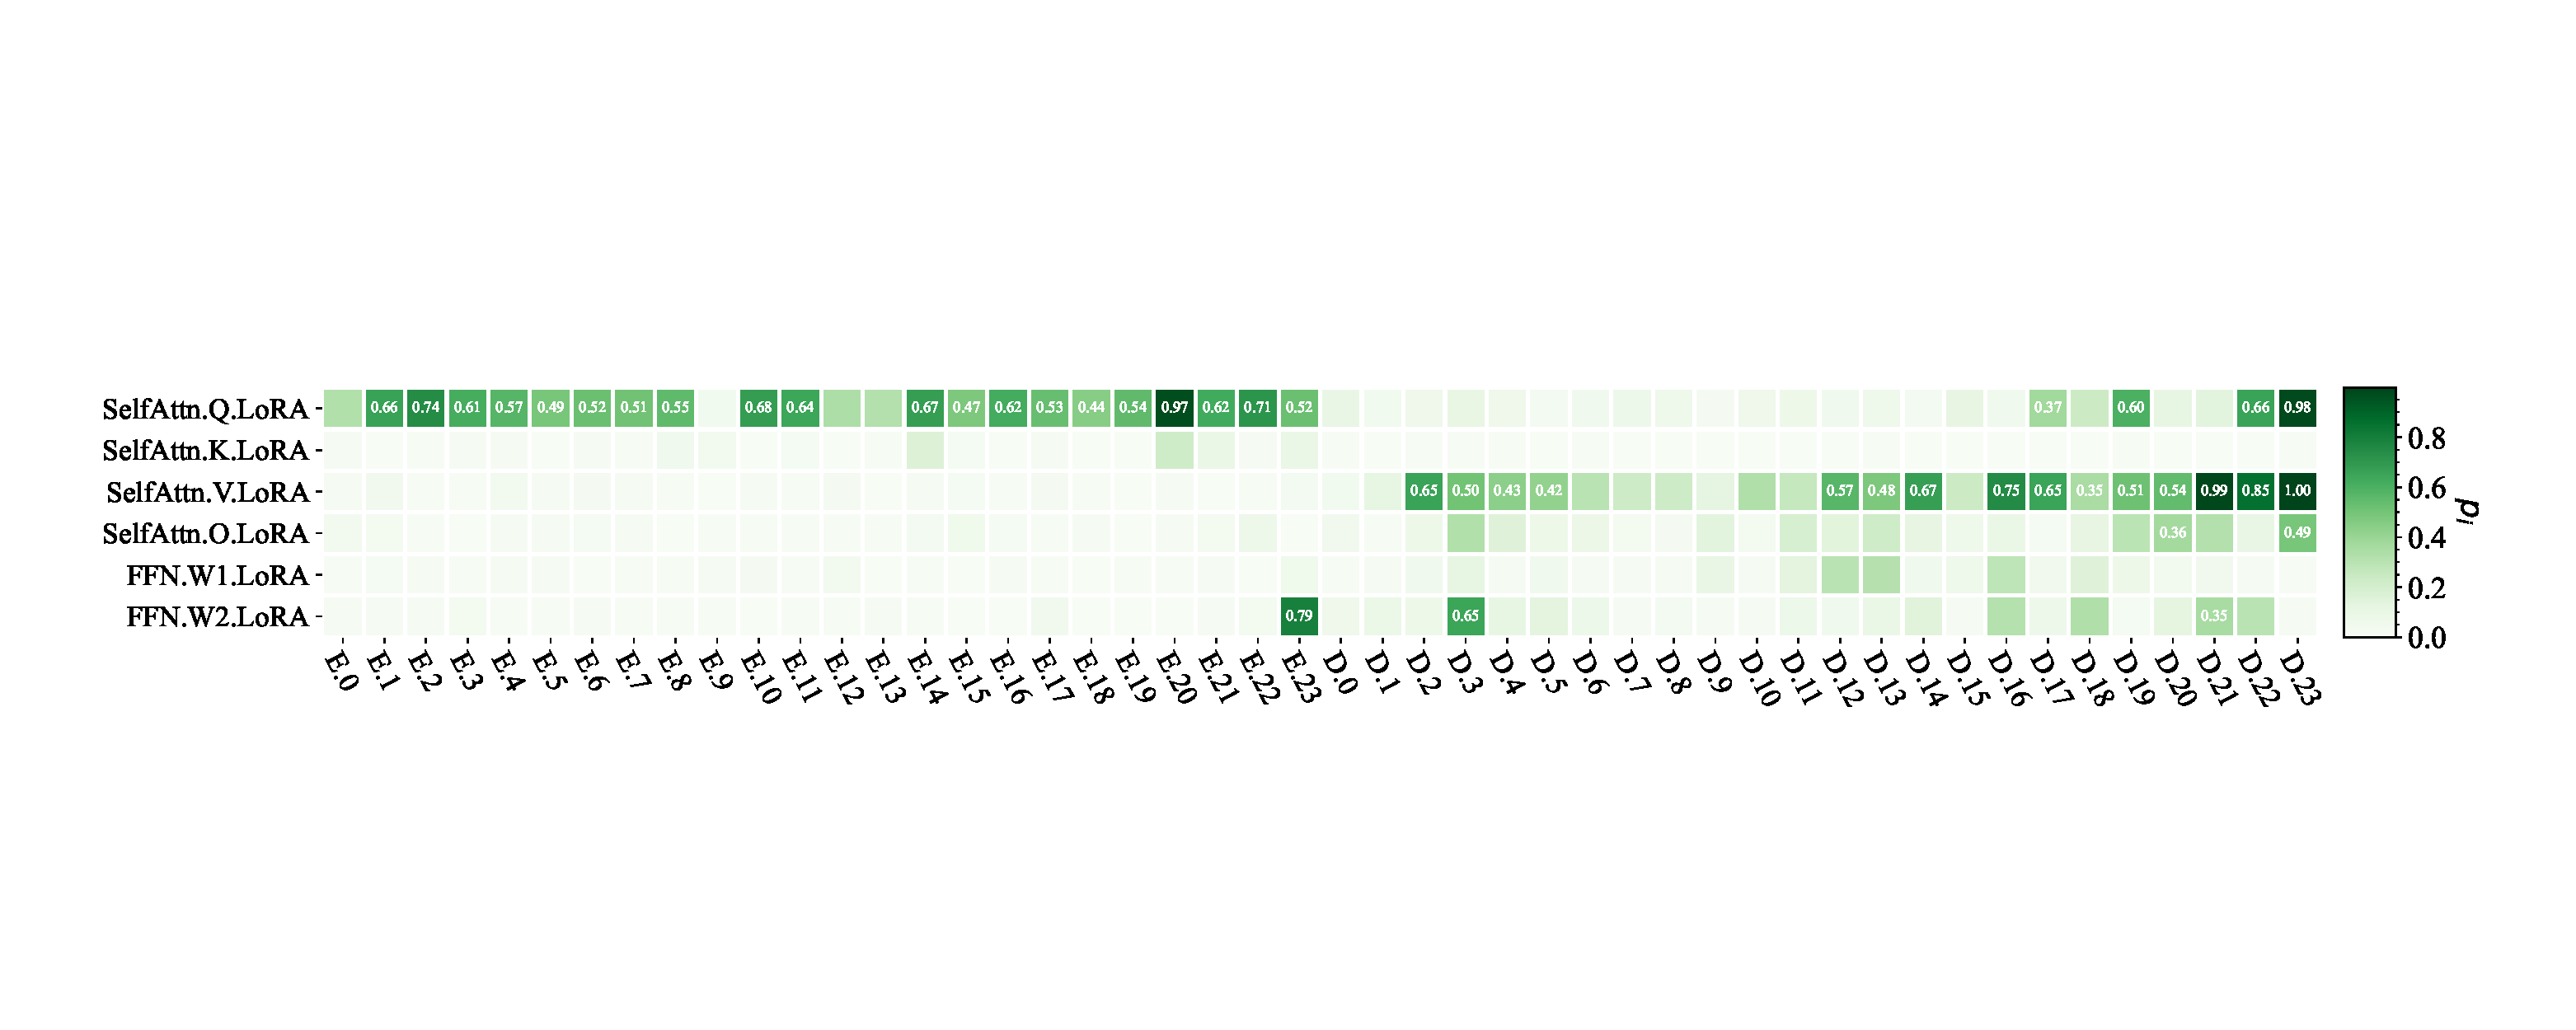
\includegraphics[width=\textwidth]{s3dfigs/heatmap_mix_1.389/superglue-wic_sparsity_1.389_heatmap.pdf}
    \vspace{-0.45cm}
    \caption{WiC}
  \end{subfigure}}
  
  \vspace{-0.3cm}
    \caption{每个数据集上 $p_i$ 的热力图}\label{app:table:all_heatmaps}
% \vspace{-1.5em}
\end{figure}